\documentclass[11pt]{article}

% --- Packages ---
\usepackage[utf8]{inputenc}
\usepackage[T1]{fontenc}
\usepackage{amsmath, amssymb, amsfonts}
\usepackage{geometry}
\usepackage{amssymb}
\usepackage{graphicx}
\usepackage{enumitem}
\usepackage{fancyhdr}
\usepackage{color}
\usepackage{hyperref}
\usepackage[most]{tcolorbox}
\usepackage{titlesec}
\usepackage{cancel} % For canceling terms
\usepackage{tikz}   % Diagrams and graphs
\usepackage{mathtools}
\usepackage{parskip}

% --- Page Setup ---
\geometry{margin=1in}
\pagestyle{fancy}
\fancyhf{}
\rhead{Algebra}
\lhead{Michael Leibbrandt}
\rfoot{\thepage}

% --- Section Styling ---
\titleformat{\section}{\large\bfseries}{\thesection}{1em}{}
\titleformat{\subsection}{\normalsize\bfseries}{\thesubsection}{1em}{}

% --- Title ---
\title{\Huge \textbf{Algebra}\\\large Notes}
\author{Michael Leibbrandt}
\date{\today}

% --- Document Begins ---
\begin{document}

\maketitle
\tableofcontents
\newpage

% ------------------------
\section{Introduction}

This document contains concise notes and worked examples.

% ------------------------
\section{Algebra Basics}

\subsection{Constants}

A \textbf{constant} is a fixed value that does not change. Unlike a \textbf{variable}, which can represent different numbers, a \textbf{constant} always has the same value.

Examples of \textbf{constant} include:

\begin{itemize}
  \item Specific numbers like \( 2 \), \( -7 \), or \( \frac{1}{2} \)
  \item Mathematical constants like \( \pi \approx 3.1416 \) or \( e \approx 2.718 \)
\end{itemize}

In the equation:
\[
x + 3 = 7
\]
the number \( 3 \) and \( 7 \) are constants — they stay the same, while \( x \) is the variable we solve for.

\subsection{Variables}

A \textbf{variable} is a symbol, usually a letter like \( x \), \( y \), or \( z \), that represents an unknown or changeable value.

For example, in the equation:
\[
x + 3 = 7
\]
the variable \( x \) represents a number. Solving the equation means finding the value of \( x \) that makes the equation true in this case, \( x = 4 \).

\textbf{Variables} are fundamental in algebra because they allow us to generalize problems and create formulas.
\subsection{Coefficients}

A \textbf{coefficient} is the numerical factor multiplied by a variable in an algebraic expression.

For example, in the term:
\[
5x
\]
the number \( 5 \) is the coefficient of the variable \( x \). It tells us how many times \( x \) is being counted or scaled.

More examples:
\begin{itemize}
  \item In \( -3y \), the coefficient is \( -3 \)
  \item In \( \frac{1}{2}a \), the coefficient is \( \frac{1}{2} \)
  \item In \( z \), the coefficient is implicitly \( 1 \), since \( z = 1 \cdot z \)
\end{itemize}

Coefficients help determine the slope of a line in linear equations and play a major role in simplifying and solving expressions.
\section{Equations vs. Expressions}

Understanding the difference between expressions and equations is essential in algebra.
\subsection{Expressions}

An \textbf{expression} is a combination of numbers, variables, and operations (like addition or multiplication), but it does \textbf{not} contain an equals sign.

Examples:
\[
2x + 5,\quad 3a^2 - 4,\quad \frac{1}{2}y
\]

Expressions represent a value, but not a complete statement to solve. You can simplify or evaluate expressions, but you cannot "solve" them unless they're part of an equation.

\subsection{Equations}

An \textbf{equation} is a mathematical statement that two expressions are equal. It always contains an equals sign (\( = \)) and usually involves finding the value of a variable that makes the equation true.

Examples:
\[
2x + 5 = 11, \quad a^2 = 16, \quad \frac{1}{2}y = 3
\]

Solving an \textbf{equation} means determining the value(s) of the variable(s) that make both sides equal.

\subsection*{Summary Table}

\begin{center}
\begin{tabular}{|c|c|}
\hline
\textbf{Expression} & \textbf{Equation} \\
\hline
No equals sign & Has an equals sign \\
Represents a value & Represents a relationship \\
Can be simplified or evaluated & Can be solved \\
Example: \( 3x + 2 \) & Example: \( 3x + 2 = 11 \) \\
\hline
\end{tabular}
\end{center}

\section{The Associative Property}

The \textbf{associative property} refers to the grouping of terms using parentheses in addition or multiplication. It tells us that the way numbers are grouped does not change the result — only the order of operations inside parentheses changes, not the outcome.

\subsection{Associative Property of Addition}

The associative property of addition states:

\[
(a + b) + c = a + (b + c)
\]

You can add numbers in any grouping, and the sum will stay the same.

\textbf{Example:}
\[
(2 + 3) + 4 = 5 + 4 = 9
\]
\[
2 + (3 + 4) = 2 + 7 = 9
\]

So, \( (2 + 3) + 4 = 2 + (3 + 4) \).

\subsection{Associative Property of Multiplication}

The associative property of multiplication states:

\[
(a \times b) \times c = a \times (b \times c)
\]

You can multiply in any grouping, and the product remains unchanged.

\textbf{Example:}
\[
(2 \times 3) \times 4 = 6 \times 4 = 24
\]
\[
2 \times (3 \times 4) = 2 \times 12 = 24
\]

So, \( (2 \times 3) \times 4 = 2 \times (3 \times 4) \).

\section{The Commutative Property}

The \textbf{commutative property} describes how the order of numbers does not affect the result when adding or multiplying. It applies only to \textbf{addition and multiplication} — not subtraction or division.

\subsection{Commutative Property of Addition}

The commutative property of addition states:

\[
a + b = b + a
\]

You can change the order of the numbers being added without changing the sum.

\textbf{Example:}
\[
4 + 7 = 11 \quad \text{and} \quad 7 + 4 = 11
\]

So, \( 4 + 7 = 7 + 4 \)

\subsection{Commutative Property of Multiplication}

The commutative property of multiplication states:

\[
a \times b = b \times a
\]

You can change the order of the numbers being multiplied without changing the product.

\textbf{Example:}
\[
6 \times 5 = 30 \quad \text{and} \quad 5 \times 6 = 30
\]

So, \( 6 \times 5 = 5 \times 6 \)
\section{Like Terms}

\textbf{Like terms} are terms that have the same variable(s) raised to the same power(s). Only the numerical coefficients can be different. Like terms can be combined using addition or subtraction.

\subsection{Addition and Subtraction of Like Terms}

To combine like terms, simply add or subtract their coefficients.

\textbf{Example 1:}
\[
3x + 5x = (3 + 5)x = 8x
\]

\textbf{Example 2:}
\[
7a^2 - 2a^2 = 5a^2
\]

\textbf{Note:} You \textit{cannot} combine terms that are not like terms.

\[
4x + 2x^2 \neq 6x^2
\quad \text{(not like terms)}
\]

\subsection{Multiplication and Division of Like Terms}

When multiplying or dividing like terms, you combine coefficients and apply exponent rules to the variables.

\textbf{Multiplication Example:}
\[
(3x)(2x) = 6x^2
\]

\[
(4a^2)(-2a^3) = -8a^5
\]

\textbf{Division Example:}
\[
\frac{10x^3}{2x} = 5x^2
\]

\[
\frac{-6y^4}{3y^2} = -2y^2
\]

\subsection*{Key Idea}

\begin{itemize}
  \item \textbf{Addition/Subtraction:} Combine only like terms (same variables and exponents)
  \item \textbf{Multiplication/Division:} Use exponent rules, even for unlike terms
\end{itemize}
\section{The Distributive Property}

The \textbf{distributive property} connects multiplication and addition or subtraction. It allows you to multiply a number or variable by each term inside parentheses.

\[
a(b + c) = ab + ac
\quad \text{and} \quad
a(b - c) = ab - ac
\]

This property is used frequently in algebra to expand expressions and solve equations.

\subsection*{Examples}

\textbf{Example 1 (with numbers):}
\[
3(4 + 5) = 3 \cdot 9 = 27
\]
\[
3 \cdot 4 + 3 \cdot 5 = 12 + 15 = 27
\]

\textbf{Example 2 (with variables):}
\[
x(2 + y) = 2x + xy
\]

\textbf{Example 3 (with subtraction):}
\[
5(a - 3) = 5a - 15
\]

\subsection*{Why It Matters}

The distributive property helps you:
\begin{itemize}
  \item Expand expressions like \( 2(x + 3) \)
  \item Simplify algebraic expressions
  \item Solve equations more efficiently
  \item Factor expressions in reverse
\end{itemize}
\subsection*{More on the Distributive Property}

The distributive property is also essential when working with variables, negative numbers, and factoring expressions.

\subsubsection*{Example with Variables and Negatives}

\[
-2(x - 4) = -2 \cdot x + (-2) \cdot (-4) = -2x + 8
\]

Notice:
\begin{itemize}
  \item The negative sign distributes to both terms
  \item Be careful with signs: \( -2 \cdot -4 = +8 \)
\end{itemize}

\subsubsection*{Common Mistake to Avoid}

Incorrect:
\[
3(x + 2) = 3x + 2 \quad \text{(Only distributed to } x \text{)}
\]

Correct:
\[
3(x + 2) = 3x + 6 \quad
\]

Always distribute to \textit{every} term inside the parentheses.

\subsubsection*{Using the Distributive Property to Factor}

The distributive property also works \textit{in reverse}, which is how we factor expressions.

\[
6x + 12 = 6(x + 2)
\]

Here, we pulled out the common factor of 6 — essentially undoing the distribution.

Factoring is the process of writing an expression as a product using the distributive property in reverse.

\textbf{Tip:} Look for a greatest common factor (GCF) before factoring!
\section{Polynomials}

A \textbf{polynomial} is an expression made up of variables, constants, and exponents, combined using addition, subtraction, and multiplication — but no variables in the denominator or under radicals.

\subsection*{Examples of Polynomials}

\[
3x^2 + 2x - 5, \quad x^3 - 4x + 7, \quad 2a^2b + 3ab^2
\]

---

\subsection{Addition and Subtraction of Polynomials}

To add or subtract polynomials:
\begin{itemize}
  \item Combine like terms (same variables raised to the same powers)
  \item Add/subtract the coefficients of like terms
\end{itemize}

\textbf{Example 1 — Addition:}
\[
(2x^2 + 3x + 1) + (x^2 + 4x - 5)
\]
\[
= (2x^2 + x^2) + (3x + 4x) + (1 - 5) = 3x^2 + 7x - 4
\]

\textbf{Example 2 — Subtraction:}
\[
(5x^2 - 2x + 6) - (3x^2 + x - 4)
\]
\[
= (5x^2 - 3x^2) + (-2x - x) + (6 + 4) = 2x^2 - 3x + 10
\]

---

\subsection{Multiplication of Polynomials}

To multiply polynomials:
\begin{itemize}
  \item Use the distributive property (FOIL for binomials)
  \item Multiply each term in the first polynomial by each term in the second
  \item Combine like terms
\end{itemize}

\textbf{Example:}
\[
(x + 2)(x + 5)
= x(x + 5) + 2(x + 5)
= x^2 + 5x + 2x + 10
= x^2 + 7x + 10
\]

\textbf{Another Example:}
\[
(2x - 3)(x^2 + x - 4)
= 2x(x^2 + x - 4) - 3(x^2 + x - 4)
\]
\[
= 2x^3 + 2x^2 - 8x - 3x^2 - 3x + 12
= 2x^3 - x^2 - 11x + 12
\]

---

\subsection{Division of Polynomials (Intro)}

Dividing polynomials can be done using:
\begin{itemize}
  \item Long division
  \item Synthetic division (when dividing by linear terms like \( x - a \))
\end{itemize}

\textbf{Basic Example:}
\[
\frac{6x^2 + 9x}{3x} = \frac{6x^2}{3x} + \frac{9x}{3x} = 2x + 3
\]

\textbf{Note:} More complex division techniques will be covered in a later section.
\begin{tcolorbox}[title=Polynomial Operations Summary, colback=blue!5!white, colframe=blue!75!black, sharp corners=southwest, boxrule=0.8pt]

\textbf{Polynomials} are expressions with variables and constants using only addition, subtraction, and multiplication (no variables in denominators or exponents).

\vspace{1ex}
\textbf{Addition/Subtraction:}
\begin{itemize}
  \item Combine like terms (same variable and exponent)
  \item Only coefficients are added or subtracted
\end{itemize}

\textbf{Multiplication:}
\begin{itemize}
  \item Use the distributive property or FOIL
  \item Multiply each term in one polynomial by each term in the other
  \item Combine like terms
\end{itemize}

\textbf{Division:}
\begin{itemize}
  \item Simplify each term if possible
  \item For complex division, use long division or synthetic division (covered later)
\end{itemize}

\end{tcolorbox}

\subsection{Long Division}

Long division is a step-by-step method for dividing numbers or algebraic expressions.

\begin{itemize}
  \item \textbf{Dividend:} the number or expression being divided
  \item \textbf{Divisor:} the number or expression you are dividing by
  \item \textbf{Quotient:} the result of the division (goes on top)
\end{itemize}

---

\subsubsection*{Example 1: Long Division with Whole Numbers}

Divide:
\[
125 \div 5
\]

Here:
\begin{itemize}
  \item Dividend = 125
  \item Divisor = 5
  \item Quotient = 25
\end{itemize}

\[
\begin{array}{r|l}
5\, &\,125 \\
\hline
& 25
\end{array}
\]

Steps:
\begin{enumerate}
  \item Divide 12 by 5 → 2 (since \( 5 \times 2 = 10 \))
  \item Subtract: \( 12 - 10 = 2 \), bring down the 5 → 25
  \item Divide 25 by 5 → 5 (since \( 5 \times 5 = 25 \))
  \item Final result: \( 25 \)
\end{enumerate}

---

\subsubsection*{Example 2: Polynomial Long Division}

Divide:
\[
\frac{x^2 + 3x + 2}{x + 1}
\]

Here:
\begin{itemize}
  \item Dividend = \( x^2 + 3x + 2 \)
  \item Divisor = \( x + 1 \)
  \item Quotient = the expression that results from division
\end{itemize}

\textbf{Step 1:} Divide leading terms:
\[
x^2 \div x = x
\]

\textbf{Step 2:} Multiply and subtract:
\[
(x^2 + 3x + 2) - (x)(x + 1) = x^2 + 3x + 2 - (x^2 + x) = 2x + 2
\]

\textbf{Step 3:} Divide leading terms again:
\[
2x \div x = 2
\]

\textbf{Step 4:} Multiply and subtract:
\[
(2x + 2) - 2(x + 1) = 2x + 2 - (2x + 2) = 0
\]

So the division is exact.

\textbf{Final Answer:}
\[
\frac{x^2 + 3x + 2}{x + 1} = x + 2
\]

---

\begin{tcolorbox}[title=Terminology Review, colback=blue!5!white, colframe=blue!75!black]
\begin{itemize}
  \item \textbf{Dividend:} what you're dividing \quad (e.g., \( x^2 + 3x + 2 \))
  \item \textbf{Divisor:} what you're dividing by \quad (e.g., \( x + 1 \))
  \item \textbf{Quotient:} result of the division \quad (e.g., \( x + 2 \))
\end{itemize}
\end{tcolorbox}
\subsection{Multivariable Polynomial Long Division}

Polynomial long division can also be performed with expressions that include more than one variable. The process is similar, but care must be taken to match like terms correctly and order terms consistently by degree.

---

\subsubsection*{Example: Divide \( 6x^2y + 9xy^2 \) by \( 3xy \)}

Here:
\begin{itemize}
  \item Dividend: \( 6x^2y + 9xy^2 \)
  \item Divisor: \( 3xy \)
\end{itemize}

\textbf{Step 1: Divide the first term of the dividend by the first term of the divisor}
\[
\frac{6x^2y}{3xy} = 2x
\]

\textbf{Step 2: Multiply the entire divisor by \( 2x \)}
\[
2x \cdot (3xy) = 6x^2y
\]

\textbf{Step 3: Subtract}
\[
(6x^2y + 9xy^2) - 6x^2y = 9xy^2
\]

\textbf{Step 4: Divide next term}
\[
\frac{9xy^2}{3xy} = 3y
\]

\textbf{Step 5: Multiply and subtract}
\[
3y \cdot (3xy) = 9xy^2
\]
\[
9xy^2 - 9xy^2 = 0
\]

\textbf{Final Answer:}
\[
\frac{6x^2y + 9xy^2}{3xy} = 2x + 3y
\]

---

\begin{tcolorbox}[title=Tips for Multivariable Long Division, colback=yellow!5!white, colframe=yellow!80!black]
\begin{itemize}
  \item Organize terms in descending order of one variable (typically \( x \))
  \item Divide one term at a time, matching both variable parts and coefficients
  \item Use standard subtraction to cancel each step before proceeding
\end{itemize}
\end{tcolorbox}
\section{Quadratic Polynomials}

A \textbf{quadratic polynomial} is a polynomial of degree 2, meaning the highest power of the variable is 2.

\subsection*{General Form}

\[
ax^2 + bx + c
\]
where:
\begin{itemize}
  \item \( a, b, c \) are real numbers and \( a \ne 0 \)
  \item \( a \) is the \textbf{leading coefficient}
  \item \( b \) is the \textbf{linear coefficient}
  \item \( c \) is the \textbf{constant term}
\end{itemize}

---

\subsection*{Examples}
\begin{itemize}
  \item \( x^2 + 5x + 6 \)
  \item \( 3x^2 - 2x + 1 \)
  \item \( -x^2 + 4 \)
\end{itemize}

---

\subsection*{Graphing Quadratics}

Quadratic functions graph as a \textbf{parabola}. The shape of the parabola depends on the sign of \( a \):
\begin{itemize}
  \item If \( a > 0 \): the parabola opens \textbf{upward} (like a smile)
  \item If \( a < 0 \): the parabola opens \textbf{downward} (like a frown)
\end{itemize}

The highest or lowest point on the parabola is called the \textbf{vertex}.

---

\subsection*{Solving Quadratic Equations}

Quadratics can be solved using several methods:
\begin{itemize}
  \item \textbf{Factoring}
  \item \textbf{Completing the square}
  \item \textbf{Quadratic formula:}
  \[
  x = \frac{-b \pm \sqrt{b^2 - 4ac}}{2a}
  \]
\end{itemize}

---

\begin{tcolorbox}[title=Quick Facts About Quadratics, colback=yellow!5!white, colframe=yellow!80!black]
\begin{itemize}
  \item Degree = 2 (because of \( x^2 \))
  \item Graph = parabola
  \item May have 0, 1, or 2 real roots depending on the discriminant \( b^2 - 4ac \)
  \item Coefficients tell you the shape and position of the graph
\end{itemize}
\end{tcolorbox}
\subsection{Factoring a Quadratic Polynomial}

Factoring is one of the most common ways to solve a quadratic equation when it can be written as a product of two binomials.

---

\subsubsection*{Example: Factor \( x^2 + 5x + 6 \)}

\textbf{Step 1:} Look for two numbers that multiply to \( 6 \) (the constant term) and add to \( 5 \) (the linear coefficient).

\[
\text{Factors of 6: } (1,6),\ (2,3)
\]
\[
2 + 3 = 5 \quad \Rightarrow \quad \text{Use } 2 \text{ and } 3
\]

\textbf{Step 2:} Write the factored form:
\[
x^2 + 5x + 6 = (x + 2)(x + 3)
\]

\textbf{Step 3:} Check by expanding:
\[
(x + 2)(x + 3) = x^2 + 3x + 2x + 6 = x^2 + 5x + 6
\]

\checkmark Confirmed!

---

\begin{tcolorbox}[title=Factoring Tips, colback=green!5!white, colframe=green!70!black]
\begin{itemize}
  \item Always look for a greatest common factor (GCF) first
  \item Use a factoring method like:
  \begin{itemize}
    \item Simple guess-and-check
    \item Box or area method
    \item AC method (for trinomials where \( a \ne 1 \))
  \end{itemize}
  \item Always double-check by expanding!
\end{itemize}
\end{tcolorbox}
\subsection{Difference of Squares}

The \textbf{difference of squares} is a special factoring pattern that applies when a binomial consists of two perfect squares being subtracted.

\[
a^2 - b^2 = (a - b)(a + b)
\]

This works because when expanded:
\[
(a - b)(a + b) = a^2 + ab - ab - b^2 = a^2 - b^2
\]

---

\subsubsection*{Examples}

\begin{itemize}
  \item \( x^2 - 9 = (x - 3)(x + 3) \)
  \item \( 4x^2 - 25 = (2x - 5)(2x + 5) \)
  \item \( 49y^2 - 1 = (7y - 1)(7y + 1) \)
  \item \(x^4 - 16 = (x^2)^2 - 4^2 = (x^2 - 4)(x^2 + 4) = (x - 2)(x + 2)(x^2 + 4) \)


\end{itemize}

---

\textbf{Important Notes:}
\begin{itemize}
  \item Works only with \textbf{subtraction}, not addition
  \item Both terms must be perfect squares
  \item Often used to simplify expressions or solve equations
\end{itemize}

---

\begin{tcolorbox}[title=Difference of Squares Summary, colback=red!5!white, colframe=red!75!black]
\[
a^2 - b^2 = (a - b)(a + b)
\]

\textbf{Examples:}
\begin{itemize}
  \item \( x^2 - 16 = (x - 4)(x + 4) \)
  \item \( 9a^2 - 1 = (3a - 1)(3a + 1) \)
\end{itemize}
\end{tcolorbox}
\subsection{Completing the Square}

To solve a quadratic equation of the form:
\[
ax^2 + bx + c = 0
\]
we can complete the square — a method that rewrites the expression as a perfect square trinomial.

---
\begin{tcolorbox}[title=What is a Trinomial?, colback=green!5!white, colframe=green!70!black]
A \textbf{trinomial} is a polynomial with three terms.

In quadratic form:
\[
ax^2 + bx + c
\]
is a trinomial.

When completing the square, we turn:
\[
x^2 + bx \quad \text{(2 terms)}
\]
into:
\[
x^2 + bx + \left( \frac{b}{2} \right)^2 \quad \text{(3 terms — a perfect square trinomial)}
\]
\end{tcolorbox}

\subsubsection*{Steps to Complete the Square (when \( a = 1 \))}

\begin{enumerate}
  \item Move the constant to the other side:
    \[
    x^2 + bx = -c
    \]
  \item Take half of the coefficient of \( x \), square it, and add to both sides:
    \[
    \left( \frac{b}{2} \right)^2
    \]
  \item Now the left-hand side is a perfect square:
    \[
    \left( x + \frac{b}{2} \right)^2
    \]
  \item Solve by taking the square root of both sides
  \item Solve for \( x \)
\end{enumerate}

---

\subsubsection*{Example: Solve \( x^2 + 6x + 4 = 0 \)}

\begin{align*}
x^2 + 6x + 4 &= 0 \\
x^2 + 6x &= -4 \\
\left( \frac{6}{2} \right)^2 &= 9 \\
x^2 + 6x + 9 &= -4 + 9 \\
(x + 3)^2 &= 5 \\
x + 3 &= \pm \sqrt{5} \\
x &= -3 \pm \sqrt{5}
\end{align*}

So the solution is:
\[
x = -3 \pm \sqrt{5}
\]

---

\begin{tcolorbox}[title=Tip for Completing the Square, colback=yellow!5!white, colframe=yellow!80!black]
\textbf{When \( a \ne 1 \)}, divide the whole equation by \( a \) first.
Completing the square is also how we derive the quadratic formula!
\end{tcolorbox}

\subsubsection*{Nature of Solutions: Real vs Complex}

After completing the square (when \( a = 1 \)), we get:
\[
x^2 + bx + c = 0 \quad \Rightarrow \quad \left(x + \frac{b}{2}\right)^2 = \left( \frac{b}{2} \right)^2 - c
\]

The number and type of solutions depend on the value of:
\[
\left( \frac{b}{2} \right)^2 - c
\]

\begin{itemize}
  \item If \( \left( \frac{b}{2} \right)^2 - c > 0 \), then \( x \) has \textbf{two real} solutions
  \item If \( \left( \frac{b}{2} \right)^2 - c = 0 \), then \( x \) has \textbf{one real} solution (a repeated root)
  \item If \( \left( \frac{b}{2} \right)^2 - c < 0 \), then \( x \) has \textbf{two complex} (nonreal) solutions
\end{itemize}

---

\begin{tcolorbox}[title=Real vs Complex Solutions from Completing the Square, colback=cyan!5!white, colframe=cyan!80!black]
Given:
\[
x^2 + bx + c = 0 \Rightarrow \left(x + \frac{b}{2} \right)^2 = \left( \frac{b}{2} \right)^2 - c
\]

Then:
\begin{itemize}
  \item \( \left( \frac{b}{2} \right)^2 - c > 0 \Rightarrow \) 2 distinct real solutions
  \item \( \left( \frac{b}{2} \right)^2 - c = 0 \Rightarrow \) 1 real solution
  \item \( \left( \frac{b}{2} \right)^2 - c < 0 \Rightarrow \) 2 complex solutions
\end{itemize}
\end{tcolorbox}
\subsubsection*{Example: Completing the Square with Imaginary Solutions}

Solve the equation:
\[
x^2 + 4x + 8 = 0
\]

\textbf{Step 1: Move the constant to the other side.}
\[
x^2 + 4x = -8
\]

\textbf{Step 2: Complete the square.}
Take half of 4 and square it:
\[
\left( \frac{4}{2} \right)^2 = 4
\]

Add 4 to both sides:
\[
x^2 + 4x + 4 = -8 + 4
\]
\[
(x + 2)^2 = -4
\]

\textbf{Step 3: Take the square root of both sides.}
\[
x + 2 = \pm \sqrt{-4}
\]
\[
x + 2 = \pm 2i
\]

\textbf{Step 4: Solve for \( x \).}
\[
x = -2 \pm 2i
\]

\textbf{Final Answer:}
\[
\boxed{x = -2 \pm 2i}
\]

---

\begin{tcolorbox}[title=Imaginary Solutions, colback=red!5!white, colframe=red!80!black]
When completing the square leads to a negative number under the square root, the equation has \textbf{two complex conjugate solutions}, involving the imaginary unit \( i = \sqrt{-1} \).
\end{tcolorbox}
\subsubsection*{Complex Conjugate Solutions and the Discriminant (When \(a=1\))}

Consider the quadratic equation:
\[
x^2 + 2x + 5 = 0
\]

Completing the square:
\[
x^2 + 2x = -5
\]
Take half of 2 and square it:
\[
\left(\frac{2}{2}\right)^2 = 1
\]
Add 1 to both sides:
\[
x^2 + 2x + 1 = -5 + 1
\]
\[
(x + 1)^2 = -4
\]

Taking the square root:
\[
x + 1 = \pm \sqrt{-4} = \pm 2i
\]

Therefore,
\[
x = -1 \pm 2i
\]

\bigskip

\textbf{Complex Conjugates:}
These solutions come in pairs called complex conjugates:
\[
a + bi \quad \text{and} \quad a - bi
\]
Here, \(a = -1\) and \(b = 2\).

\bigskip

\textbf{Discriminant:}
The discriminant is:
\[
\Delta = b^2 - 4ac
\]
For the equation:
\[
a = 1, \quad b = 2, \quad c = 5
\]
\[
\Delta = 2^2 - 4 \cdot 1 \cdot 5 = 4 - 20 = -16 < 0
\]

Since \(\Delta < 0\), the solutions are complex conjugates.

\begin{tcolorbox}[title=Summary, colback=cyan!5!white, colframe=cyan!80!black]
\begin{itemize}
  \item \(\Delta > 0\): Two distinct real solutions
  \item \(\Delta = 0\): One repeated real solution
  \item \(\Delta < 0\): Two complex conjugate solutions
\end{itemize}
\end{tcolorbox}
\subsection*{The Quadratic Formula and the Discriminant}

Any quadratic equation of the form:
\[
ax^2 + bx + c = 0
\]
can be solved using the \textbf{quadratic formula}:
\[
x = \frac{-b \pm \sqrt{b^2 - 4ac}}{2a}
\]

\bigskip

\textbf{Discriminant:}
The expression under the square root, denoted by:
\[
\Delta = b^2 - 4ac
\]
is called the \textbf{discriminant}. It determines the type of solutions:

\begin{tcolorbox}[title=Discriminant Summary, colback=yellow!5!white, colframe=yellow!80!black]
\begin{itemize}
  \item If \( \Delta > 0 \): two distinct real solutions
  \item If \( \Delta = 0 \): one real solution (a repeated root)
  \item If \( \Delta < 0 \): two complex conjugate solutions
\end{itemize}
\end{tcolorbox}

\bigskip

\textbf{Example:}
Solve \( x^2 - 2x - 3 = 0 \) using the quadratic formula.

Here, \(a = 1\), \(b = -2\), and \(c = -3\).
Compute the discriminant:
\[
\Delta = (-2)^2 - 4(1)(-3) = 4 + 12 = 16
\]

Now apply the formula:
\[
x = \frac{-(-2) \pm \sqrt{16}}{2(1)} = \frac{2 \pm 4}{2}
\]

So the two solutions are:
\[
x = \frac{2 + 4}{2} = 3 \quad \text{and} \quad x = \frac{2 - 4}{2} = -1
\]

\bigskip

\textbf{Conclusion:}
The quadratic formula is a universal method for solving any quadratic equation, and the discriminant tells you what kind of solutions to expect.
\section{The Cartesian Plane}

The Cartesian Plane is a two-dimensional coordinate system defined by a horizontal number line called the \textbf{x-axis}, and a vertical number line called the \textbf{y-axis}. These axes intersect at the \textbf{origin}, denoted as \( (0, 0) \).

Each point on the plane is represented by an ordered pair \( (x, y) \), where:
\begin{itemize}
  \item \( x \) is the horizontal value (left/right),
  \item \( y \) is the vertical value (up/down).
\end{itemize}

\begin{center}
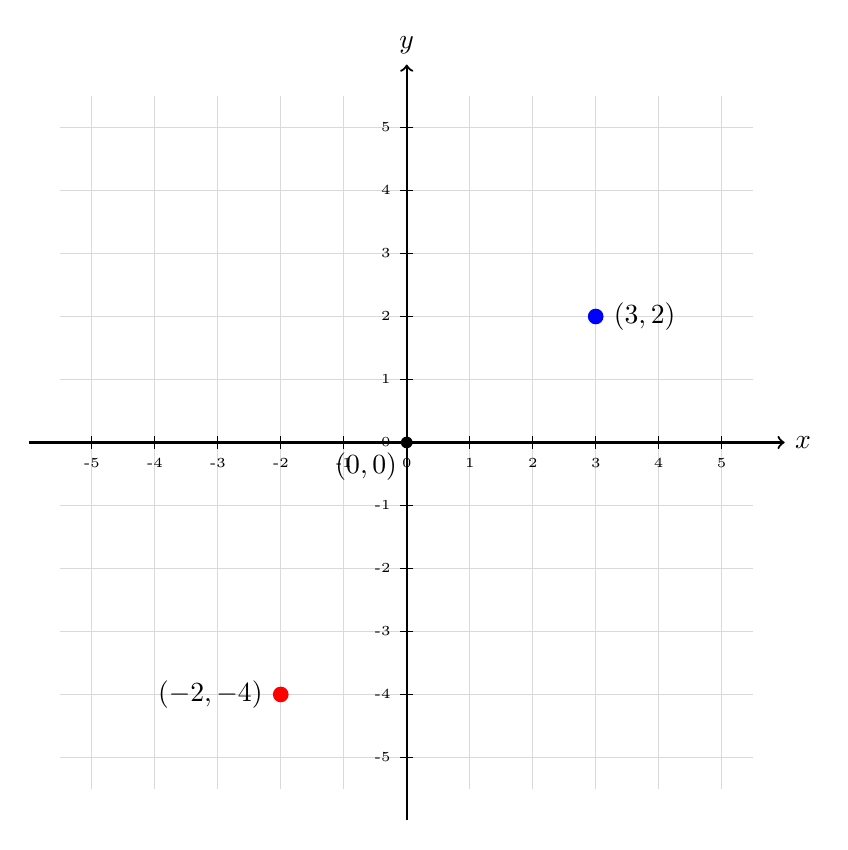
\begin{tikzpicture}[scale=0.8]
  \draw[very thin,color=gray!30] (-5.5,-5.5) grid (5.5,5.5);
  \draw[->,thick] (-6,0) -- (6,0) node[right] {\( x \)};
  \draw[->,thick] (0,-6) -- (0,6) node[above] {\( y \)};
  \node at (0,0) [circle,fill=black,inner sep=1.5pt]{};
  \node[below left] at (0,0) {\( (0, 0) \)};
  \foreach \x in {-5,-4,...,5} {
    \draw (\x,0.1) -- (\x,-0.1) node[below] {\tiny \x};
  }
  \foreach \y in {-5,-4,...,5} {
    \draw (0.1,\y) -- (-0.1,\y) node[left] {\tiny \y};
  }
  \node[circle,fill=blue,inner sep=2pt,label={right:\( (3,2) \)}] at (3,2) {};
  \node[circle,fill=red,inner sep=2pt,label={left:\( (-2,-4) \)}] at (-2,-4) {};
\end{tikzpicture}
\end{center}

\begin{tcolorbox}[colback=blue!5!white, colframe=blue!75!black, title=Summary]
\begin{itemize}
  \item The Cartesian Plane has two axes: \( x \)-axis (horizontal), \( y \)-axis (vertical).
  \item The point where they meet is the origin \( (0, 0) \).
  \item Each point is identified by an ordered pair (Called a coordinate) \( (x, y) \).
\end{itemize}
\end{tcolorbox}
\subsection{The Four Quadrants}

The Cartesian Plane is divided into four regions called \textbf{quadrants}. These are numbered in a counterclockwise direction starting from the upper-right:

\begin{itemize}
  \item \textbf{Quadrant I}: \( (+x, +y) \)
  \item \textbf{Quadrant II}: \( (-x, +y) \)
  \item \textbf{Quadrant III}: \( (-x, -y) \)
  \item \textbf{Quadrant IV}: \( (+x, -y) \)
\end{itemize}

\begin{center}
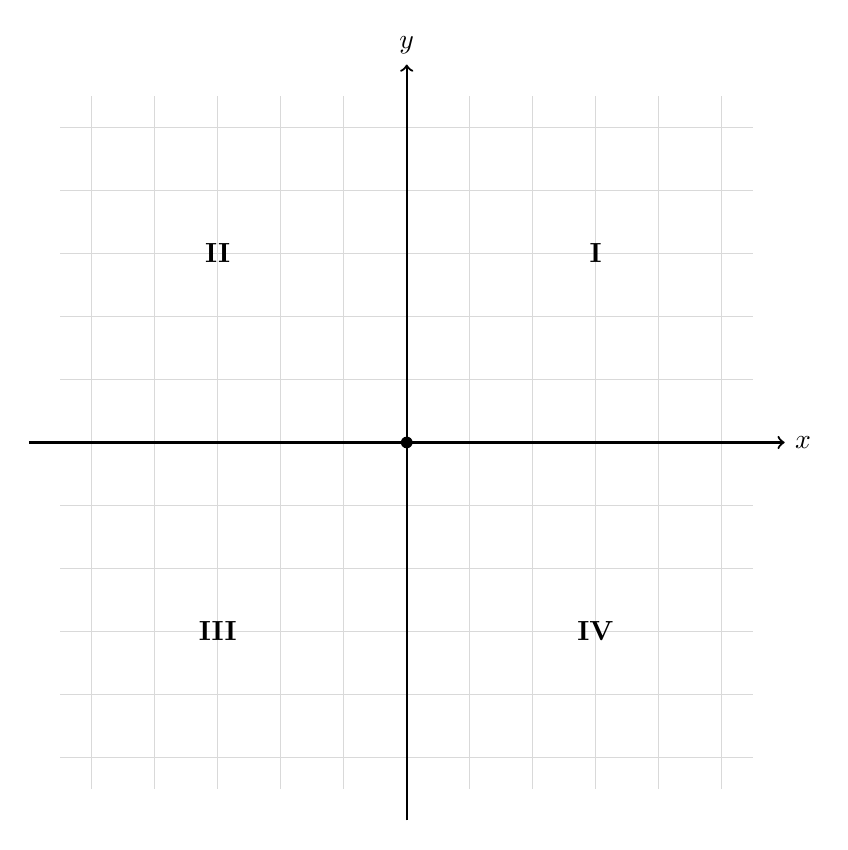
\begin{tikzpicture}[scale=0.8]
  \draw[very thin,color=gray!30] (-5.5,-5.5) grid (5.5,5.5);
  \draw[->,thick] (-6,0) -- (6,0) node[right] {\( x \)};
  \draw[->,thick] (0,-6) -- (0,6) node[above] {\( y \)};
  \node at (0,0) [circle,fill=black,inner sep=1.5pt]{};
  \node at (3,3) {\textbf{I}};
  \node at (-3,3) {\textbf{II}};
  \node at (-3,-3) {\textbf{III}};
  \node at (3,-3) {\textbf{IV}};
\end{tikzpicture}
\end{center}

\begin{tcolorbox}[colback=green!5!white, colframe=green!50!black, title=Summary of Quadrants]
\begin{itemize}
  \item Points in each quadrant have characteristic signs for \(x\) and \(y\).
  \item The quadrants are labeled I through IV, moving counterclockwise.
\end{itemize}
\end{tcolorbox}
\subsection{Slope of a Line}

The \textbf{slope} of a line is a measure of its steepness. It tells us how much the \( y \)-value changes for a given change in the \( x \)-value.

Given two points on a line, \( (x_1, y_1) \) and \( (x_2, y_2) \), the slope \( m \) is calculated using the formula:

\[
m = \frac{y_2 - y_1}{x_2 - x_1}
\]

This is also known as “rise over run”:
\begin{itemize}
  \item \textbf{Rise}: the vertical change \( (y_2 - y_1) \)
  \item \textbf{Run}: the horizontal change \( (x_2 - x_1) \)
\end{itemize}

\begin{center}
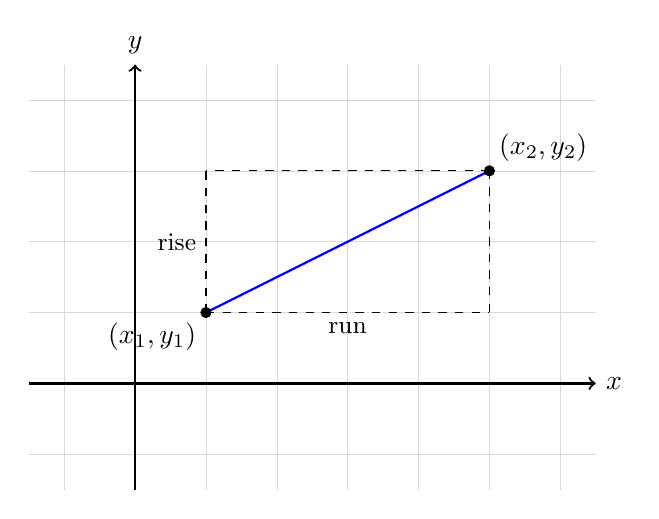
\begin{tikzpicture}[scale=0.9]
  \draw[very thin,color=gray!30] (-1.5,-1.5) grid (6.5,4.5);
  \draw[->,thick] (-1.5,0) -- (6.5,0) node[right] {\( x \)};
  \draw[->,thick] (0,-1.5) -- (0,4.5) node[above] {\( y \)};
  \coordinate (A) at (1,1);
  \coordinate (B) at (5,3);
  \draw[thick,blue] (A) -- (B);
  \filldraw[black] (A) circle (2pt) node[below left] {\( (x_1, y_1) \)};
  \filldraw[black] (B) circle (2pt) node[above right] {\( (x_2, y_2) \)};
  \draw[dashed] (A) -- ++(4,0) node[midway,below] {\small run};
  \draw[dashed] (B) -- ++(-4,0);
  \draw[dashed] (A) -- ++(0,2) node[midway,left] {\small rise};
  \draw[dashed] (B) -- ++(0,-2);
\end{tikzpicture}
\end{center}

\begin{tcolorbox}[colback=yellow!5!white, colframe=yellow!80!black, title=Summary: Slope of a Line]
\begin{itemize}
  \item Slope measures how steep a line is.
  \item Use \( m = \dfrac{y_2 - y_1}{x_2 - x_1} \) to calculate it.
  \item A positive slope rises left to right; negative slope falls.
\end{itemize}
\end{tcolorbox}

\subsection{Point-Slope Form of a Line}

If you know the slope \( m \) of a line and a point \( (x_1, y_1) \) it passes through, you can write the line's equation using the \textbf{point-slope form}:

\[
y - y_1 = m(x - x_1)
\]

\textbf{Requirements:}
\begin{itemize}
  \item A single point \( (x_1, y_1) \)
  \item The slope \( m \)
\end{itemize}

\textbf{Example:}
Given the point \( (2, 3) \) and slope \( m = 4 \), the equation becomes:

\[
y - 3 = 4(x - 2)
\]

This can be left in point-slope form or simplified to slope-intercept form.

\begin{tcolorbox}[colback=cyan!5!white, colframe=cyan!80!black, title=Point-Slope Summary]
\begin{itemize}
  \item Use when you know one point and the slope.
  \item Formula: \( y - y_1 = m(x - x_1) \)
\end{itemize}
\end{tcolorbox}

\subsection{Slope-Intercept Form of a Line}

The \textbf{slope-intercept form} expresses a linear equation as:

\[
y = mx + b
\]

Where:
\begin{itemize}
  \item \( m \) is the slope of the line.
  \item \( b \) is the \textbf{y-intercept} — the value of \( y \) when \( x = 0 \).
\end{itemize}

\textbf{Requirements:}
\begin{itemize}
  \item Slope \( m \)
  \item Y-intercept \( b \)
\end{itemize}

\textbf{Example:}
If a line has slope \( m = -2 \) and y-intercept \( b = 5 \), the equation is:

\[
y = -2x + 5
\]

This form is especially useful for graphing.

\begin{tcolorbox}[colback=orange!5!white, colframe=orange!80!black, title=Slope-Intercept Summary]
\begin{itemize}
  \item Use when slope and y-intercept are known.
  \item Formula: \( y = mx + b \)
  \item \( b \) tells you where the line crosses the \( y \)-axis.
\end{itemize}
\end{tcolorbox}
\subsection{Converting Between Forms of a Linear Equation}

Linear equations can be written in multiple forms. It’s often helpful to convert between them depending on the context (e.g., graphing, solving, or analyzing).

\subsubsection*{1. Point-Slope to Slope-Intercept}

Start with the point-slope form:
\[
y - y_1 = m(x - x_1)
\]

Distribute the slope and solve for \( y \) to convert to slope-intercept form:
\begin{align*}
y - y_1 &= m(x - x_1) \\
y &= m(x - x_1) + y_1 \quad \text{(Slope-Intercept Form: \( y = mx + b \))}
\end{align*}

\textbf{Example:}
Convert \( y - 2 = 3(x + 1) \) to slope-intercept form:
\begin{align*}
y - 2 &= 3(x + 1) \\
y - 2 &= 3x + 3 \\
y &= 3x + 5
\end{align*}

\subsubsection*{2. Two Points to Any Form}

Given two points \( (x_1, y_1) \) and \( (x_2, y_2) \):
\begin{enumerate}
  \item Find the slope \( m = \dfrac{y_2 - y_1}{x_2 - x_1} \)
  \item Use point-slope form with one point
  \item Convert to slope-intercept form if needed
\end{enumerate}

\begin{tcolorbox}[colback=purple!5!white, colframe=purple!80!black, title=Summary: Converting Forms]
\begin{itemize}
  \item Point-slope to slope-intercept: distribute and solve for \( y \)
  \item Two points → slope → point-slope → slope-intercept
  \item Use the form that best suits the problem (graphing, solving, etc.)
\end{itemize}
\end{tcolorbox}
\subsection{Undefined Slope and Vertical Lines}

A \textbf{vertical line} goes straight up and down and has an \textbf{undefined slope}. This is because its run (change in \( x \)) is zero:

\[
m = \frac{y_2 - y_1}{x_2 - x_1}
\]

If \( x_2 = x_1 \), then the denominator becomes 0, and division by zero is undefined.

\section*{Equation of a Vertical Line:}
A vertical line through \( x = a \) is written as:

\[
x = a
\]

\begin{itemize}
  \item It has an \textbf{undefined slope}.
  \item It has an \textbf{x-intercept only} — it does not cross the \( y \)-axis.
\end{itemize}

\begin{center}
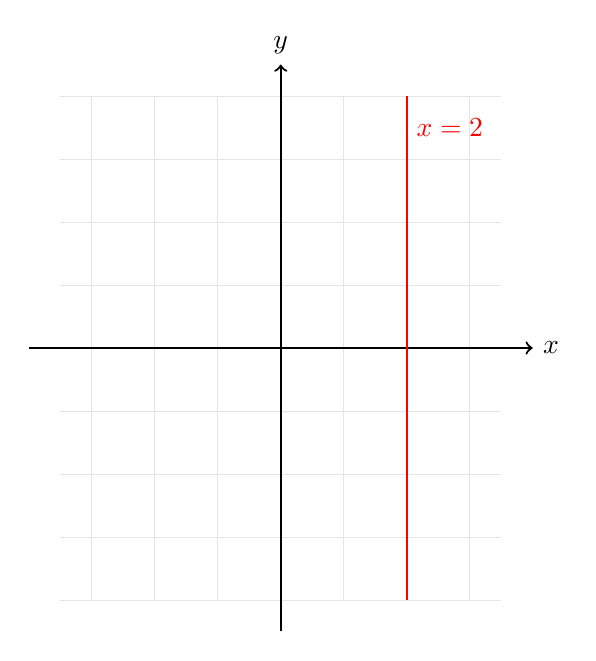
\begin{tikzpicture}[scale=0.8]
  \draw[very thin,color=gray!20] (-3.5,-4) grid (3.5,4);
  \draw[->,thick] (-4,0) -- (4,0) node[right] {\( x \)};
  \draw[->,thick] (0,-4.5) -- (0,4.5) node[above] {\( y \)};
  \draw[thick,red] (2,-4) -- (2,4);
  \node[red,right] at (2,3.5) {\( x = 2 \)};
\end{tikzpicture}
\end{center}

\begin{tcolorbox}[colback=red!5!white, colframe=red!80!black, title=Important Notes on Vertical Lines]
\begin{itemize}
  \item Vertical lines have the form \( x = a \)
  \item Their slope is undefined.
  \item They do not cross the \( y \)-axis — no \( y \)-intercept exists.
\end{itemize}
\end{tcolorbox}
\section{Graphing Linear Equations}

To graph a linear equation, such as:

\[
y = mx + b
\]

you can create a \textbf{table of values} by plugging in values for \( x \) and solving for \( y \). This gives you a set of points you can plot on the Cartesian plane.

\subsection*{Steps to Graph a Line}
\begin{enumerate}
  \item Choose three \( x \)-values (commonly: \( -1, 0, 1 \))
  \item Plug them into the equation to find corresponding \( y \)-values
  \item Plot the points \( (x, y) \) on the graph
  \item Draw a straight line through the points
\end{enumerate}

\subsection*{Example: Graph \( y = 2x + 1 \)}

\textbf{Step 1: Create a table}

\[
\begin{array}{c|c}
x & y = 2x + 1 \\
\hline
-1 & 2(-1) + 1 = -2 + 1 = -1 \\
0 & 2(0) + 1 = 0 + 1 = 1 \\
1 & 2(1) + 1 = 2 + 1 = 3 \\
\end{array}
\]

\textbf{Step 2: Plot points}

\[
(-1, -1), \quad (0, 1), \quad (1, 3)
\]

\textbf{Step 3: Draw a straight line through the points}

\begin{center}
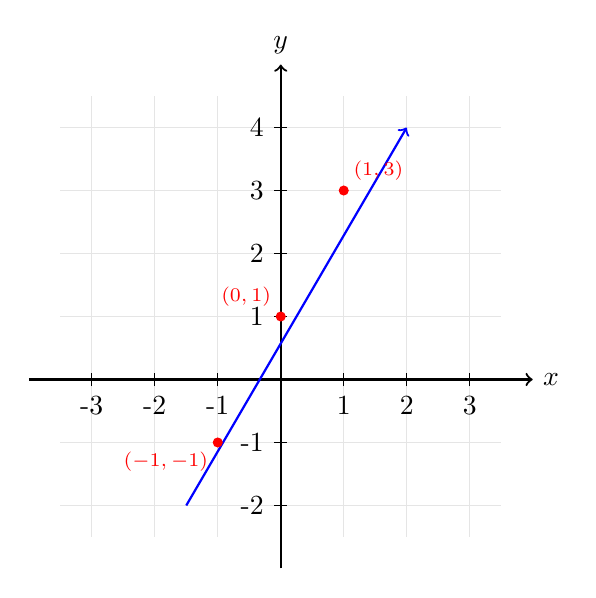
\begin{tikzpicture}[scale=0.8]
  \draw[very thin,color=gray!20] (-3.5,-2.5) grid (3.5,4.5);
  \draw[->,thick] (-4,0) -- (4,0) node[right] {\( x \)};
  \draw[->,thick] (0,-3) -- (0,5) node[above] {\( y \)};
  \foreach \x in {-3,-2,-1,1,2,3}
    \draw[shift={(\x,0)},color=black] (0pt,-3pt) -- (0pt,3pt) node[below=5pt] {\x};
  \foreach \y in {-2,-1,1,2,3,4}
    \draw[shift={(0,\y)},color=black] (-3pt,0pt) -- (3pt,0pt) node[left=5pt] {\y};

  \draw[thick,blue,->] (-1.5,-2) -- (2,4);
  \filldraw[red] (-1,-1) circle (2pt) node[below left] {\scriptsize$(-1, -1)$};
  \filldraw[red] (0,1) circle (2pt) node[above left] {\scriptsize$(0, 1)$};
  \filldraw[red] (1,3) circle (2pt) node[above right] {\scriptsize$(1, 3)$};
\end{tikzpicture}
\end{center}

\begin{tcolorbox}[colback=blue!5!white, colframe=blue!80!black, title=Graphing Summary]
\begin{itemize}
  \item Pick easy \( x \)-values: \( -1, 0, 1 \)
  \item Solve for \( y \), make a table
  \item Plot at least 3 points and draw the line
\end{itemize}
\end{tcolorbox}

\section{Functions}

A \textbf{function} is a relation where each input has exactly one output. The input is called the \textbf{independent variable} (usually \( x \)), and the output is the \textbf{dependent variable} (usually \( y \)).

Formally, a function \( f \) from a set \( A \) (domain) to a set \( B \) (codomain) assigns each element \( x \in A \) to exactly one element \( y \in B \), written as:
\[
y = f(x)
\]

\bigskip

\textbf{Key points about functions:}
\begin{itemize}
  \item For every \( x \), there is \emph{only one} corresponding \( y \).
  \item The value of \( y \) depends on the choice of \( x \).
  \item Functions can be represented by equations, tables, graphs, or mappings.
\end{itemize}

\bigskip

\textbf{Example:} Consider the function
\[
f(x) = 2x + 3.
\]
To find the output when \( x = 4 \), substitute \( 4 \) into the function:
\[
f(4) = 2(4) + 3 = 8 + 3 = 11.
\]
So, the function value at \( x = 4 \) is 11.

\bigskip

\textbf{Function notation:}
\[
f(x) = y
\]
means "the value of the function \( f \) at input \( x \) is \( y \)."


\subsection{Not a Function}

An equation is \textbf{not a function} if one input has \emph{multiple outputs}. You can test this with the \textbf{vertical line test} — if a vertical line touches the graph in more than one place, it is \emph{not} a function.

\textbf{Examples of equations that are not functions:}
\begin{itemize}
  \item \( x = 3 \) — a vertical line (undefined slope)
  \item \( x^2 + y^2 = 1 \) — a circle (one \( x \) leads to two \( y \) values)
\end{itemize}

\begin{center}
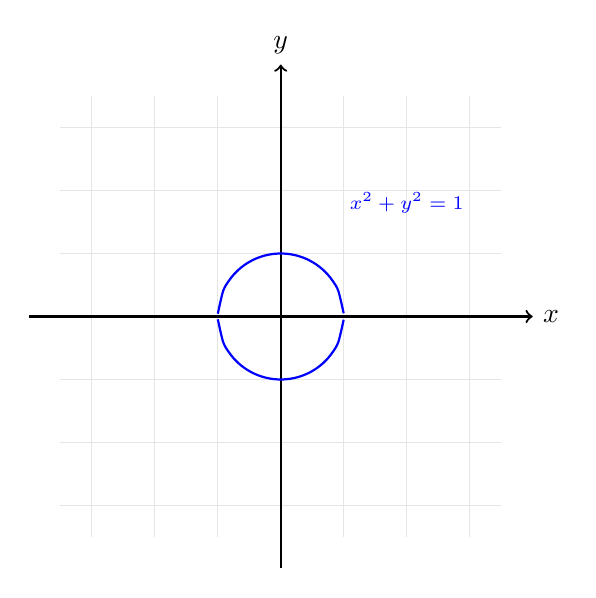
\begin{tikzpicture}[scale=0.8]
  \draw[very thin,color=gray!20] (-3.5,-3.5) grid (3.5,3.5);
  \draw[->,thick] (-4,0) -- (4,0) node[right] {\( x \)};
  \draw[->,thick] (0,-4) -- (0,4) node[above] {\( y \)};

  % Circle (Not a function)
  \draw[thick,blue,domain=-0.999:0.999,smooth,variable=\x]
  plot ({\x},{sqrt(1 - \x*\x)});
\draw[thick,blue,domain=-0.999:0.999,smooth,variable=\x]
  plot ({\x},{-sqrt(1 - \x*\x)});
  \node[blue] at (2,1.8) {\scriptsize \( x^2 + y^2 = 1 \)};
\end{tikzpicture}
\end{center}

\begin{tcolorbox}[colback=purple!5!white, colframe=purple!80!black, title=Function Summary]
\begin{itemize}
  \item A function gives exactly one output for each input.
  \item It passes the \textbf{vertical line test}.
  \item Not all equations are functions!
\end{itemize}
\end{tcolorbox}

\subsection{Domain and Range}

\textbf{Domain:} The set of all possible input values (\( x \)) for which the function is defined.

\textbf{Range:} The set of all possible output values (\( y \)) that the function can produce.

\bigskip

\textbf{How to find Domain and Range:}

\begin{itemize}
  \item \textbf{Given a function \( f(x) \):}
  Analyze the equation to determine which \( x \)-values are allowed. For example, avoid division by zero or square roots of negative numbers.

  \medskip

  \item \textbf{Given a set of points:}
  The domain is the set of all \( x \)-coordinates, and the range is the set of all \( y \)-coordinates.

  \medskip

  \item \textbf{Given a graph:}
  - The domain corresponds to all \( x \)-values covered by the graph (horizontally).
  - The range corresponds to all \( y \)-values covered by the graph (vertically).
\end{itemize}

\bigskip

\textbf{Example:}

Consider the function
\[
f(x) = \sqrt{x - 2}.
\]

\begin{itemize}
  \item \textbf{Domain:} Since the expression inside the square root must be non-negative,
  \[
  x - 2 \geq 0 \implies x \geq 2,
  \]
  so the domain is \( [2, \infty) \).

  \item \textbf{Range:} The square root outputs non-negative values, so
  \[
  y \geq 0,
  \]
  and the range is \( [0, \infty) \).
\end{itemize}

\subsection{Is It a Function? (Testing Sets of Values)}

To determine if a relation (a set of ordered pairs or an equation) is a function, use the following rule:

\begin{tcolorbox}[colback=yellow!5!white, colframe=yellow!80!black, title=Function Test]
A relation is a \textbf{function} if \emph{every input} (\( x \)-value) corresponds to \emph{exactly one output} (\( y \)-value).
\end{tcolorbox}

\textbf{Example 1 (Function — Set of Points):}
\[
\{ (1, 2), (2, 3), (3, 4) \}
\]
Each input is unique — this \textbf{is} a function.

\medskip

\textbf{Example 2 (Not a Function — Set of Points):}
\[
\{ (1, 2), (1, 3), (2, 4) \}
\]
The input \( 1 \) maps to two different outputs (\( 2 \) and \( 3 \)) — this is \textbf{not} a function.

\bigskip

\textbf{Example 3 (Algebraic Test):}

Consider the equation:
\[
x^2 + y^2 = 1
\]

Solve for \( y \):
\[
y^2 = 1 - x^2 \Rightarrow y = \pm \sqrt{1 - x^2}
\]

This gives two \( y \)-values for a single \( x \)-value.
\textbf{Conclusion:} This is \textbf{not} a function.

\bigskip

\textbf{Steps to check:}
\begin{enumerate}
  \item List all \( x \)-values or solve for \( y \).
  \item If any \( x \)-value gives more than one \( y \), it's \textbf{not} a function.
\end{enumerate}

\section{Operations with Functions}

\subsection{Sum of Functions}

The \textbf{sum of two functions} means adding their outputs for the same input value.

\begin{tcolorbox}[colback=blue!5!white, colframe=blue!80!black, title=Sum of Functions]
If \( f(x) \) and \( g(x) \) are two functions, then:
\[
(f + g)(x) = f(x) + g(x)
\]
This means you add the two expressions for each value of \( x \).
\end{tcolorbox}

\subsubsection*{Example}

Let:
\[
f(x) = 2x + 3 \quad \text{and} \quad g(x) = x^2 - 1
\]

Then:
\[
(f + g)(x) = f(x) + g(x) = (2x + 3) + (x^2 - 1)
\]

Simplify:
\[
(f + g)(x) = x^2 + 2x + 2
\]

\subsubsection*{Evaluation Example}

Find \( (f + g)(2) \):

\begin{align*}
f(2) &= 2(2) + 3 = 7 \\
g(2) &= (2)^2 - 1 = 3 \\
(f + g)(2) &= f(2) + g(2) = 7 + 3 = 10
\end{align*}

\subsection{Adding Functions from Sets of Points}

You can also add two functions given as sets of ordered pairs. Just add the \( y \)-values for matching \( x \)-values.

\begin{tcolorbox}[colback=green!5!white, colframe=green!50!black, title=Adding Point-Based Functions]
If:
\[
f = \{ (1, 2), (2, 4), (3, 6) \}, \quad g = \{ (1, 5), (2, 1), (3, -2) \}
\]

Then:
\[
(f + g)(x) = \{ (1, 2+5), (2, 4+1), (3, 6+(-2)) \} = \{ (1, 7), (2, 5), (3, 4) \}
\]
\end{tcolorbox}

\textbf{Note:} This only works when both functions share the same \( x \)-values.
\subsection{Product of Functions}

The \textbf{product of two functions} means multiplying their outputs for each input value.

\begin{tcolorbox}[colback=yellow!5!white, colframe=yellow!80!black, title=Product of Functions]
If \( f(x) \) and \( g(x) \) are functions, then:
\[
(f \cdot g)(x) = f(x) \cdot g(x)
\]
This means you multiply their expressions together.
\end{tcolorbox}

\subsubsection*{Example (Algebraic Expressions)}

Let:
\[
f(x) = 2x + 1, \quad g(x) = x - 3
\]

Then:
\[
(f \cdot g)(x) = f(x) \cdot g(x) = (2x + 1)(x - 3)
\]

Use distribution (FOIL):
\[
(f \cdot g)(x) = 2x^2 - 6x + x - 3 = 2x^2 - 5x - 3
\]

\subsubsection*{Evaluation Example}

Find \( (f \cdot g)(2) \):

\begin{align*}
f(2) &= 2(2) + 1 = 5 \\
g(2) &= 2 - 3 = -1 \\
(f \cdot g)(2) &= 5 \cdot (-1) = -5
\end{align*}

\subsubsection{Product from Sets of Points}

If:
\[
f = \{ (1, 2), (2, 4), (3, 6) \}, \quad g = \{ (1, 5), (2, 1), (3, -2) \}
\]

Then:
\[
(f \cdot g)(x) = \{ (1, 2 \cdot 5), (2, 4 \cdot 1), (3, 6 \cdot (-2)) \} = \{ (1, 10), (2, 4), (3, -12) \}
\]

\textbf{Note:} Only valid if the \( x \)-values match in both functions.

\subsection{Even, Odd, or Neither}

To classify a function as \textbf{even}, \textbf{odd}, or \textbf{neither}, evaluate \( f(-x) \) and compare it to \( f(x) \) and \( -f(x) \):

\begin{tcolorbox}[colback=blue!5!white, colframe=blue!80!black, title=Function Symmetry Rules]
\begin{itemize}
  \item \textbf{Even:} \( f(-x) = f(x) \) — symmetric about the \textbf{y-axis}
  \item \textbf{Odd:} \( f(-x) = -f(x) \) — symmetric about the \textbf{origin}
  \item \textbf{Neither:} \( f(-x) \ne f(x) \) and \( f(-x) \ne -f(x) \)
\end{itemize}
\end{tcolorbox}

---

\subsubsection*{Even Function — \( f(x) = x^2 \)}

\begin{minipage}{0.45\textwidth}
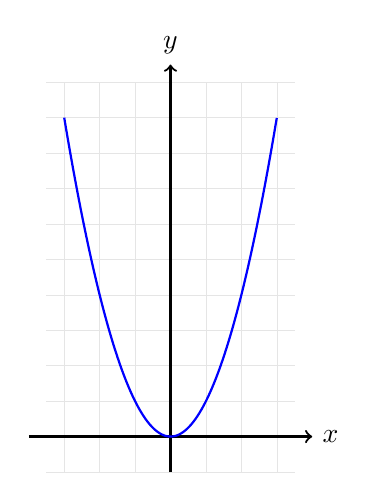
\begin{tikzpicture}[scale=0.45]
  \draw[very thin,color=gray!20] (-3.5,-1) grid (3.5,10);
  \draw[->,thick] (-4,0) -- (4,0) node[right] {\( x \)};
  \draw[->,thick] (0,-1) -- (0,10.5) node[above] {\( y \)};
  \draw[thick,blue,domain=-3:3,smooth,samples=100] plot (\x,{(\x)^2});
\end{tikzpicture}
\end{minipage}
\begin{minipage}{0.5\textwidth}
\textbf{Table of values:}
\begin{center}
\begin{tabular}{|c|c|}
\hline
\( x \) & \( f(x) \) \\
\hline
-2 & 4 \\
-1 & 1 \\
0  & 0 \\
1  & 1 \\
2  & 4 \\
\hline
\end{tabular}
\end{center}
\end{minipage}

---

\subsubsection*{Odd Function — \( f(x) = x^3 \)}

\begin{minipage}{0.45\textwidth}
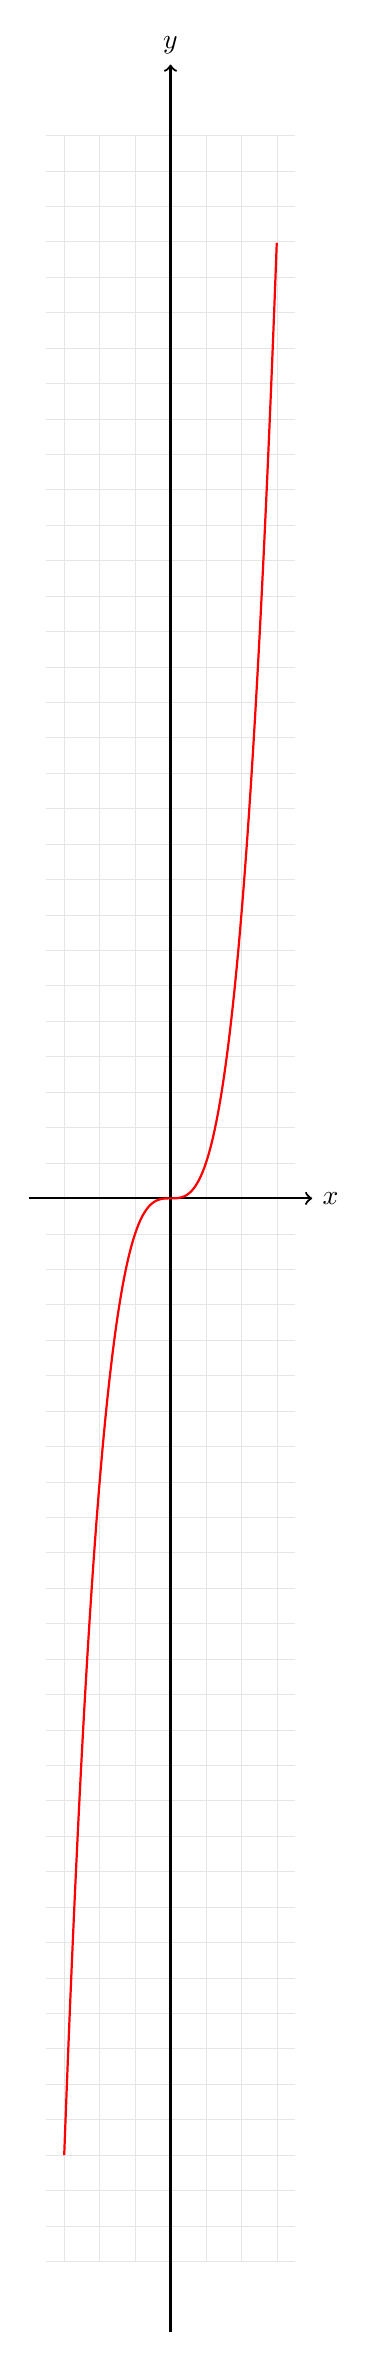
\begin{tikzpicture}[scale=0.45]
  \draw[very thin,color=gray!20] (-3.5,-30) grid (3.5,30);
  \draw[->,thick] (-4,0) -- (4,0) node[right] {\( x \)};
  \draw[->,thick] (0,-32) -- (0,32) node[above] {\( y \)};
  \draw[thick,red,domain=-3:3,smooth,samples=100] plot (\x,{(\x)^3});
\end{tikzpicture}
\end{minipage}
\begin{minipage}{0.5\textwidth}
\textbf{Table of values:}
\begin{center}
\begin{tabular}{|c|c|}
\hline
\( x \) & \( f(x) \) \\
\hline
-2 & -8 \\
-1 & -1 \\
0  & 0 \\
1  & 1 \\
2  & 8 \\
\hline
\end{tabular}
\end{center}
\end{minipage}

---

\subsubsection*{Neither — \( f(x) = x^2 + x \)}

\begin{minipage}{0.45\textwidth}
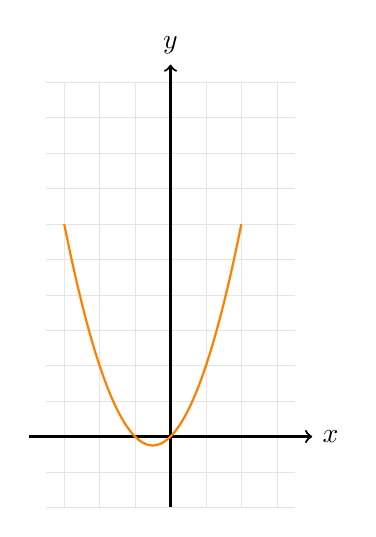
\begin{tikzpicture}[scale=0.45]
  \draw[very thin,color=gray!20] (-3.5,-2) grid (3.5,10);
  \draw[->,thick] (-4,0) -- (4,0) node[right] {\( x \)};
  \draw[->,thick] (0,-2) -- (0,10.5) node[above] {\( y \)};
  \draw[thick,orange,domain=-3:2,smooth,samples=100] plot (\x,{(\x)^2 + \x});
\end{tikzpicture}
\end{minipage}
\begin{minipage}{0.5\textwidth}
\textbf{Why is it neither?}
\[
f(-x) = x^2 - x \ne f(x) \text{ and } \ne -f(x)
\]
No symmetry about the y-axis or origin.
\end{minipage}

---

\subsubsection*{Quick Summary}

\begin{itemize}
  \item \textbf{Even:} Symmetric about the \( y \)-axis (e.g., \( x^2 \))
  \item \textbf{Odd:} Symmetric about the origin (e.g., \( x^3 \))
  \item \textbf{Neither:} Fails both tests (e.g., \( x^2 + x \))
\end{itemize}
\section{Trichotomy}

\subsection*{The Trichotomy Property}

The \textbf{Trichotomy Property} states that for any real number \( a \), exactly one of the following is true:

\begin{itemize}
  \item \( a > 0 \) (positive)
  \item \( a = 0 \) (zero)
  \item \( a < 0 \) (negative)
\end{itemize}

This property applies to all real numbers and ensures that any number must fall into one — and only one — of these categories.

\begin{tcolorbox}[colback=cyan!5!white, colframe=cyan!80!black, title=Trichotomy Summary]
For any real number \( a \), exactly one of the following holds:
\[
a > 0 \quad \text{or} \quad a = 0 \quad \text{or} \quad a < 0
\]
Only one condition can be true at a time.
\end{tcolorbox}

\subsubsection*{Examples}

\begin{itemize}
  \item \( 7 > 0 \): Positive
  \item \( 0 = 0 \): Zero
  \item \( -5 < 0 \): Negative
\end{itemize}

\subsubsection*{Why It Matters}

Trichotomy is fundamental in:
\begin{itemize}
  \item Solving inequalities
  \item Proving properties in algebra and calculus
  \item Understanding number line positioning
\end{itemize}

\section*{Inequalities and Negative Numbers}

\subsection{Working with Inequalities}

Inequalities show relationships between two values using symbols:

\begin{itemize}
  \item \( < \): less than
  \item \( > \): greater than
  \item \( \leq \): less than or equal to
  \item \( \geq \): greater than or equal to
\end{itemize}

\subsection{Multiplying or Dividing by Negatives}

When you \textbf{multiply or divide} both sides of an inequality by a \textbf{negative number}, you must \textbf{reverse the direction} of the inequality.

\begin{tcolorbox}[colback=orange!5!white, colframe=orange!80!black, title=Important Rule]
If you multiply or divide both sides of an inequality by a negative number, the inequality sign flips:
\[
\text{If } a < b \text{, then } -a > -b
\]
\end{tcolorbox}

\subsubsection*{Examples}

\begin{itemize}
  \item Original: \( 3 < 5 \)
    Multiply both sides by \( -1 \):
    \( -3 > -5 \)
  \item Solve: \( -2x > 6 \)
    Divide both sides by \( -2 \):
    \( x < -3 \) (Notice the sign flip!)
\end{itemize}

\subsection*{Why This Happens}

Negative numbers reverse order on the number line. For example:
\[
-3 > -5 \quad \text{because } -3 \text{ is to the right of } -5
\]

\begin{tcolorbox}[colback=yellow!5!white, colframe=yellow!80!black, title=Summary]
\begin{itemize}
  \item Inequalities describe relative size.
  \item Operations like addition and subtraction don’t flip the sign.
  \item Multiplying or dividing by a \textbf{negative} \emph{does}.
\end{itemize}
\end{tcolorbox}

\subsection{Graphing Inequalities on a Number Line}

To graph inequalities, we use a number line with:
\begin{itemize}
  \item An \textbf{open circle} for \( < \) or \( > \) (value is \emph{not} included)
  \item A \textbf{closed (filled) circle} for \( \leq \) or \( \geq \) (value \emph{is} included)
  \item An arrow to indicate all values greater than or less than the point
\end{itemize}

\subsubsection*{Examples}

\begin{center}
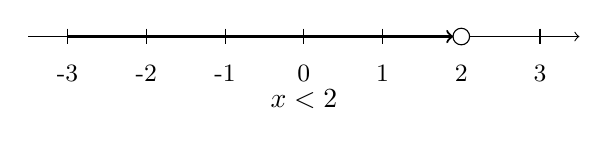
\begin{tikzpicture}
  % x < 2
  \draw[->] (-3.5,0) -- (3.5,0);
  \foreach \x in {-3,...,3}
    \draw (\x,0.1) -- (\x,-0.1) node[below=4pt] {\small \x};
  \draw[fill=white,draw=black] (2,0) circle (3pt);
  \draw[thick,->] (-3,0) -- (1.9,0);
  \node at (0,-0.8) {\( x < 2 \)};
\end{tikzpicture}
\end{center}

\begin{center}
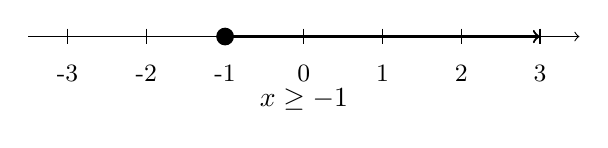
\begin{tikzpicture}
  % x ≥ -1
  \draw[->] (-3.5,0) -- (3.5,0);
  \foreach \x in {-3,...,3}
    \draw (\x,0.1) -- (\x,-0.1) node[below=4pt] {\small \x};
  \draw[fill=black] (-1,0) circle (3pt);
  \draw[thick,->] (-0.9,0) -- (3,0);
  \node at (0,-0.8) {\( x \geq -1 \)};
\end{tikzpicture}
\end{center}

\begin{tcolorbox}[colback=blue!5!white, colframe=blue!80!black, title=Summary]
\begin{itemize}
  \item Use \textbf{open circles} for strict inequalities (\( < \), \( > \))
  \item Use \textbf{closed circles} for inclusive inequalities (\( \leq \), \( \geq \))
  \item Shade to the left for "less than", and to the right for "greater than"
\end{itemize}
\end{tcolorbox}

\subsection{Graphing Disjunctions (OR)}

A \textbf{disjunction} connects two inequalities with "or" (symbol: \(\lor\)).
The solution includes values that satisfy \emph{either} inequality.

\begin{itemize}
  \item Graph both inequalities separately.
  \item Shade all values that satisfy \emph{either} one.
  \item The graph is the \textbf{union} of both solution sets.
\end{itemize}

\subsubsection*{Example:}

\[
x < -1 \quad \lor \quad x > 2
\]

\begin{center}
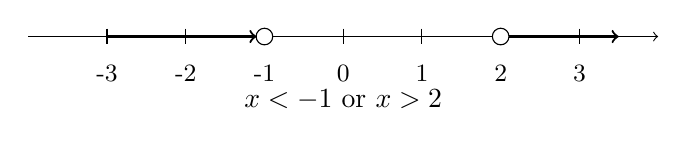
\begin{tikzpicture}
  \draw[->] (-4,0) -- (4,0);
  \foreach \x in {-3,...,3}
    \draw (\x,0.1) -- (\x,-0.1) node[below=4pt] {\small \x};
  \draw[fill=white] (-1,0) circle (3pt);
  \draw[thick,->] (-3,0) -- (-1.1,0);
  \draw[fill=white] (2,0) circle (3pt);
  \draw[thick,->] (2.1,0) -- (3.5,0);
  \node at (0,-0.8) {\( x < -1 \text{ or } x > 2 \)};
\end{tikzpicture}
\end{center}

\vspace{1em}

\subsection{Graphing Conjunctions (AND)}

A \textbf{conjunction} connects two inequalities with "and" (symbol: \(\land\)).
The solution includes values that satisfy \emph{both} inequalities simultaneously.

\begin{itemize}
  \item Graph both inequalities separately.
  \item The solution is the \textbf{intersection} of the two graphs.
  \item Shade only where both overlap.
\end{itemize}

\subsubsection*{Example:}

\[
-2 \leq x < 3
\]

This can be written as the conjunction:

\[
x \geq -2 \quad \land \quad x < 3
\]

\begin{center}
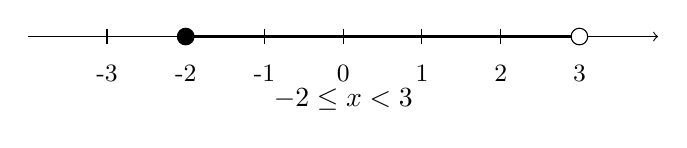
\begin{tikzpicture}
  \draw[->] (-4,0) -- (4,0);
  \foreach \x in {-3,...,3}
    \draw (\x,0.1) -- (\x,-0.1) node[below=4pt] {\small \x};
  \draw[fill=black] (-2,0) circle (3pt);
  \draw[fill=white] (3,0) circle (3pt);
  \draw[thick] (-2,0) -- (2.9,0);
  \node at (0,-0.8) {\( -2 \leq x < 3 \)};
\end{tikzpicture}
\end{center}

\begin{tcolorbox}[colback=cyan!5!white, colframe=cyan!80!black, title=Summary]
\begin{itemize}
  \item \textbf{Disjunction (OR)} solutions combine all values satisfying either inequality.
  \item \textbf{Conjunction (AND)} solutions are values satisfying both inequalities simultaneously.
  \item On number lines, OR means shading the union, AND means shading the intersection.
\end{itemize}
\end{tcolorbox}

\subsection{Graphing Inequalities in the Plane}

To graph a linear inequality in two variables (like \( y < 2x + 1 \)), follow these steps:

\begin{enumerate}
  \item \textbf{Graph the boundary line:}
  Replace the inequality symbol with an equals sign and graph the resulting line:
  \[
  y = 2x + 1
  \]
  Use a \textbf{dashed line} for \( < \) or \( > \), and a \textbf{solid line} for \( \leq \) or \( \geq \).

  \item \textbf{Choose a test point:}
  Often the point \( (0, 0) \) is easiest. Plug it into the inequality to check if it makes the inequality true.

  \item \textbf{Shade the correct region:}
  If the test point satisfies the inequality, shade the side of the line that includes it. Otherwise, shade the opposite side.
\end{enumerate}

\subsubsection*{Example: \( y < 2x + 1 \)}

\begin{center}
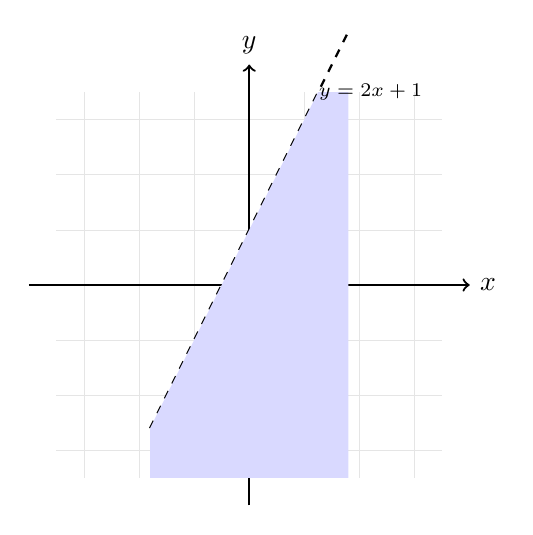
\begin{tikzpicture}[scale=0.7]
  % Grid and axes
  \draw[very thin,color=gray!20] (-3.5,-3.5) grid (3.5,3.5);
  \draw[->,thick] (-4,0) -- (4,0) node[right] {\(x\)};
  \draw[->,thick] (0,-4) -- (0,4) node[above] {\(y\)};

  % Dashed boundary line: y = 2x + 1
  \draw[dashed,thick,domain=-1.8:1.8] plot (\x,{2*\x + 1});

  % Shaded region below the line
  \begin{scope}
    \clip (-3.5,-3.5) rectangle (3.5,3.5);
    \fill[blue!15, domain=-1.8:1.8, variable=\x]
      plot ({\x}, {2*\x + 1}) --
      (1.8,-3.5) -- (-1.8,-3.5) -- cycle;
  \end{scope}

  % Label
  \node at (2.2,3.5) {\scriptsize \( y = 2x + 1 \)};
\end{tikzpicture}
\end{center}

\begin{tcolorbox}[colback=orange!5!white, colframe=orange!80!black, title=Tips]
\begin{itemize}
  \item Dashed line: inequality does \textbf{not include} the boundary (e.g., \( < \), \( > \))
  \item Solid line: inequality \textbf{includes} the boundary (e.g., \( \leq \), \( \geq \))
  \item Shade the region where the inequality holds true.
\end{itemize}
\end{tcolorbox}

\section{Absolute Value Equations}

Absolute value equations involve expressions within absolute value bars, such as:

\[
|f(x)| = a
\]

\begin{tcolorbox}[colback=blue!5!white, colframe=blue!75!black, title=General Cases]
\begin{itemize}
  \item If \( a > 0 \), then there are \textbf{two solutions}: \( f(x) = a \) or \( f(x) = -a \)
  \item If \( a = 0 \), then there is \textbf{one solution}: \( f(x) = 0 \)
  \item If \( a < 0 \), then there are \textbf{no solutions}, because absolute value is never negative.
\end{itemize}
\end{tcolorbox}

\subsubsection*{Example 1: \( |x - 4| = 6 \)}

Solve:
\begin{align*}
x - 4 &= 6 \quad \text{or} \quad x - 4 = -6 \\
x &= 10 \quad \text{or} \quad x = -2
\end{align*}

\subsubsection*{Example 2: \( |2x + 5| = 0 \)}

\begin{align*}
2x + 5 &= 0 \\
x &= -\frac{5}{2}
\end{align*}

\subsubsection*{Example 3: \( |x + 3| = -7 \)}

\textbf{No solution}, because the absolute value can’t equal a negative number.

\begin{tcolorbox}[colback=purple!5!white, colframe=purple!80!black, title=Summary]
\begin{itemize}
  \item Isolate the absolute value expression.
  \item Set up two equations: one positive, one negative.
  \item Check for invalid cases (e.g., equals a negative number).
\end{itemize}
\end{tcolorbox}

\subsection{Absolute Value Inequalities}

Absolute value inequalities involve comparisons such as:

\[
|f(x)| < a \quad \text{or} \quad |f(x)| > a
\]

\begin{tcolorbox}[colback=orange!5!white, colframe=orange!75!black, title=Key Cases]
\begin{enumerate}
  \item \textbf{\( |f(x)| < \text{(negative)} \)} \\
    \hspace{1em}No solution — absolute value is always non-negative.

  \item \textbf{\( |f(x)| > \text{(negative)} \)} \\
    \hspace{1em}All real numbers — all absolute values are greater than any negative number.

  \item \textbf{\( |f(x)| < a \)} (where \( a > 0 \)) \\
    \hspace{1em}\textbf{Conjunction:} Rewrite as a compound inequality:
    \[
    -a < f(x) < a
    \]

  \item \textbf{\( |f(x)| > a \)} (where \( a > 0 \)) \\
    \hspace{1em}\textbf{Disjunction:} Split into two separate inequalities:
    \[
    f(x) < -a \quad \text{or} \quad f(x) > a
    \]
\end{enumerate}
\end{tcolorbox}

\subsubsection*{Example 1: \( |x - 2| < 5 \)}

\begin{align*}
-5 &< x - 2 < 5 \\
-3 &< x < 7
\end{align*}

\subsubsection*{Example 2: \( |x + 4| > 3 \)}

\begin{align*}
x + 4 &< -3 \quad \text{or} \quad x + 4 > 3 \\
x &< -7 \quad \text{or} \quad x > -1
\end{align*}

\section{Solving Systems of Equations}

A \textbf{system of equations} consists of two or more equations with the same set of variables. A solution to the system is the point(s) where the equations intersect — that is, the values that satisfy all equations simultaneously.

There are three common methods to solve a system of linear equations:

\subsection{1. Substitution Method}

\textbf{Steps:}
\begin{enumerate}
  \item Solve one equation for one variable.
  \item Substitute this expression into the other equation.
  \item Solve for the remaining variable.
  \item Plug back in to find the other variable.
\end{enumerate}

\textbf{Example:}
\[
\begin{aligned}
y &= 2x + 1 \\
3x + y &= 13
\end{aligned}
\]

Substitute \( y = 2x + 1 \) into the second equation:
\[
3x + (2x + 1) = 13 \Rightarrow 5x = 12 \Rightarrow x = \frac{12}{5}
\]
Then find \( y \):
\[
y = 2\left(\frac{12}{5}\right) + 1 = \frac{24}{5} + \frac{5}{5} = \frac{29}{5}
\]

\subsection{2. Elimination Method}

\textbf{Steps:}
\begin{enumerate}
  \item Align equations and eliminate one variable by addition or subtraction.
  \item Solve for the remaining variable.
  \item Substitute back to find the other variable.
\end{enumerate}

\textbf{Example:}
\[
\begin{aligned}
2x + 3y &= 7 \\
4x - 3y &= 5
\end{aligned}
\]

Add the two equations:
\[
(2x + 3y) + (4x - 3y) = 7 + 5 \Rightarrow 6x = 12 \Rightarrow x = 2
\]

Substitute \( x = 2 \) into the first equation:
\[
2(2) + 3y = 7 \Rightarrow 4 + 3y = 7 \Rightarrow y = 1
\]

\subsection{3. Graphing Method}

\textbf{Steps:}
\begin{enumerate}
  \item Graph both equations on the same coordinate plane.
  \item Identify the point of intersection.
\end{enumerate}

\textbf{Example:}
\[
\begin{aligned}
y &= x + 1 \\
y &= -x + 5
\end{aligned}
\]

Graph both lines. The intersection point is:
\[
x + 1 = -x + 5 \Rightarrow 2x = 4 \Rightarrow x = 2, \quad y = 3
\]

\textbf{Solution: } \( (2, 3) \)

\begin{tcolorbox}[colback=blue!5!white, colframe=blue!80!black, title=System of Equations Summary]
\begin{itemize}
  \item \textbf{Substitution:} Use when one equation is already solved for a variable.
  \item \textbf{Elimination:} Use when variables align easily for cancellation.
  \item \textbf{Graphing:} Use to visualize solutions — intersection point is the solution.
\end{itemize}
\end{tcolorbox}
\subsection{Solving Systems of Linear Inequalities (Graphing)}

A \textbf{system of linear inequalities} consists of two or more inequalities. The solution is the region where all the shaded areas (solutions to each inequality) \textbf{overlap}.

\textbf{Steps to Graph:}
\begin{enumerate}
  \item Graph each inequality as if it were an equation (\( y = mx + b \)).
  \item Use a \textbf{dashed line} for \( < \) or \( > \), and a \textbf{solid line} for \( \leq \) or \( \geq \).
  \item Shade the correct side of the line:
  \begin{itemize}
    \item Use a test point (like \( (0, 0) \)) to see which side satisfies the inequality.
  \end{itemize}
  \item Repeat for each inequality.
  \item The \textbf{solution region} is where all shaded areas overlap.
\end{enumerate}

\textbf{Example:}
\[
\begin{cases}
y \leq 2x + 1 \\
y > -x + 3
\end{cases}
\]

\begin{center}
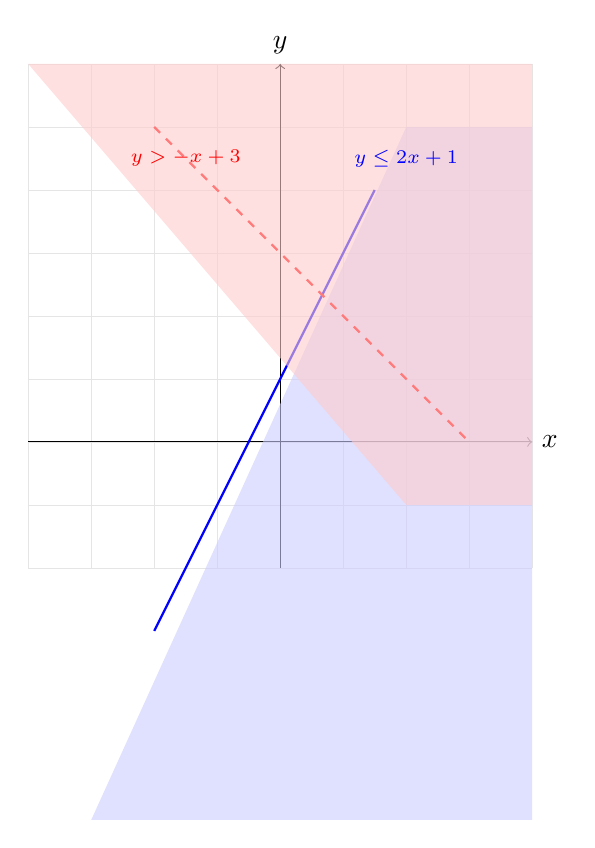
\begin{tikzpicture}[scale=0.8]
  \draw[very thin,color=gray!20] (-4,-2) grid (4,6);
  \draw[->] (-4,0) -- (4,0) node[right] {\(x\)};
  \draw[->] (0,-2) -- (0,6) node[above] {\(y\)};

  % y = 2x + 1 (solid line)
  \draw[domain=-2:1.5,thick,blue] plot (\x,{2*\x+1});
  \fill[blue!20,opacity=0.6] (-3,-6) -- (2,5) -- (4,5) -- (4,-6) -- cycle;

  % y = -x + 3 (dashed line)
  \draw[domain=-2:3,thick,red,dashed] plot (\x,{-\x+3});
  \fill[red!20,opacity=0.6] (-4,6) -- (2,-1) -- (4,-1) -- (4,6) -- cycle;

  \node[blue] at (2,4.5) {\scriptsize \( y \leq 2x + 1 \)};
  \node[red] at (-1.5,4.5) {\scriptsize \( y > -x + 3 \)};
\end{tikzpicture}
\end{center}

\begin{tcolorbox}[colback=green!5!white, colframe=green!80!black, title=Graphing Systems of Inequalities]
\begin{itemize}
  \item The \textbf{solution set} is the region where all shaded areas \textbf{intersect}.
  \item Use \textbf{solid lines} for \( \leq, \geq \); \textbf{dashed lines} for \( <, > \).
  \item Always test with a point if you're unsure which side to shade.
\end{itemize}
\end{tcolorbox}
\section{Exponents and Special Powers}

\subsection*{Powers of Negative Bases}

When a negative number is raised to a power, the result depends on whether the exponent is even or odd:

\begin{itemize}
  \item \textbf{Even Exponent:} Negative base raised to an even power gives a \textbf{positive} result.
    \[
    (-2)^4 = 16
    \]
  \item \textbf{Odd Exponent:} Negative base raised to an odd power gives a \textbf{negative} result.
    \[
    (-2)^3 = -8
    \]
  \item \textbf{Important:} Be careful with parentheses.
    \[
    -2^4 = -(2^4) = -16 \quad \text{(Not the same as } (-2)^4 \text{)}
    \]
\end{itemize}

\subsection*{Negative Exponents}

A negative exponent represents a reciprocal:
\[
a^{-n} = \frac{1}{a^n}, \quad a \neq 0
\]
\begin{itemize}
  \item Example:
    \[
    2^{-3} = \frac{1}{2^3} = \frac{1}{8}
    \]
  \item Applies to variables as well:
    \[
    x^{-2} = \frac{1}{x^2}, \quad x \neq 0
    \]
\end{itemize}

\subsection*{Zero Exponent}

Any nonzero number raised to the power of zero equals 1:
\[
a^0 = 1, \quad a \neq 0
\]
\begin{itemize}
  \item Example:
    \[
    5^0 = 1 \quad\text{and}\quad (-3)^0 = 1
    \]
  \item Note: \( 0^0 \) is considered \textbf{undefined}.
\end{itemize}

\begin{tcolorbox}[colback=yellow!5!white, colframe=yellow!80!black, title=Exponent Rules Summary]
\begin{itemize}
  \item \( (-a)^n \): Positive if \( n \) is even, negative if \( n \) is odd.
  \item \( a^{-n} = \frac{1}{a^n} \) — Negative exponent means reciprocal.
  \item \( a^0 = 1 \), as long as \( a \neq 0 \).
\end{itemize}
\end{tcolorbox}

\section{Fractional Exponents}

\subsection*{What is a Fractional Exponent?}

A fractional exponent represents a \textbf{root}. The general rule is:

\[
a^{\frac{m}{n}} = \sqrt[n]{a^m} = \left( \sqrt[n]{a} \right)^m
\]

\textbf{Special case:}
\[
a^{\frac{1}{n}} = \sqrt[n]{a}
\]

\begin{itemize}
  \item The \textbf{denominator} (\( n \)) of the fraction tells you the \textbf{root}.
  \item The \textbf{numerator} (\( m \)) tells you the \textbf{power}.
\end{itemize}

\subsection*{Examples}

\begin{align*}
  9^{\frac{1}{2}} &= \sqrt{9} = 3 \\
  8^{\frac{1}{3}} &= \sqrt[3]{8} = 2 \\
  16^{\frac{3}{4}} &= \left( \sqrt[4]{16} \right)^3 = 2^3 = 8 \\
  27^{\frac{2}{3}} &= \left( \sqrt[3]{27} \right)^2 = 3^2 = 9
\end{align*}

\begin{tcolorbox}[colback=cyan!5!white, colframe=cyan!80!black, title=Fractional Exponents Summary]
\begin{itemize}
  \item \( a^{\frac{1}{n}} = \sqrt[n]{a} \)
  \item \( a^{\frac{m}{n}} = \sqrt[n]{a^m} = \left( \sqrt[n]{a} \right)^m \)
  \item Fractional exponents are just another way to express roots and powers.
\end{itemize}
\end{tcolorbox}

\subsection{Product Property of Radicals}

The \textbf{Product Property of Radicals} states that:

\[
\sqrt{a} \cdot \sqrt{b} = \sqrt{ab}
\quad \text{where } a \geq 0,\, b \geq 0
\]

This property allows you to multiply square roots by combining the radicands into a single radical.

\begin{tcolorbox}[colback=blue!5!white, colframe=blue!75!black, title=Product Property of Radicals]
\[
\sqrt[n]{a} \cdot \sqrt[n]{b} = \sqrt[n]{ab}
\quad \text{(for } a, b \geq 0 \text{ and } n \in \mathbb{N},\, n \geq 2 \text{)}
\]
\end{tcolorbox}

\textbf{Examples:}
\begin{itemize}
  \item \( \sqrt{3} \cdot \sqrt{12} = \sqrt{36} = 6 \)
  \item \( \sqrt[3]{2} \cdot \sqrt[3]{4} = \sqrt[3]{8} = 2 \)
\end{itemize}

\textbf{Note:} This rule does \textbf{not} apply to negative radicands when working within the real numbers.


\section{Rationalizing the Denominator}

Sometimes, we encounter expressions where the denominator contains a square root or an irrational number. Rationalizing the denominator means rewriting the expression so that there are \textbf{no radicals in the denominator}.

\vspace{1em}

\subsection*{Why Rationalize?}
Rationalizing helps simplify expressions for further operations and provides a standard form that’s easier to compare or graph.

\subsection*{Case 1: Single Radical in the Denominator}

\begin{tcolorbox}[colback=blue!5!white, colframe=blue!80!black, title=Example: Single Radical]
Simplify:
\[
\frac{3}{\sqrt{2}}
\]

Multiply numerator and denominator by \( \sqrt{2} \):
\[
\frac{3}{\sqrt{2}} \cdot \frac{\sqrt{2}}{\sqrt{2}} = \frac{3\sqrt{2}}{2}
\]
\end{tcolorbox}

\subsection*{Case 2: Binomial with a Radical (Use the Conjugate)}

When the denominator is a binomial with a radical, multiply by the conjugate:
\[
\text{Conjugate of } a + \sqrt{b} \text{ is } a - \sqrt{b}
\]

\begin{tcolorbox}[colback=purple!5!white, colframe=purple!80!black, title=Example: Binomial Denominator]
Simplify:
\[
\frac{5}{3 + \sqrt{2}}
\]

Multiply by the conjugate:
\[
\frac{5}{3 + \sqrt{2}} \cdot \frac{3 - \sqrt{2}}{3 - \sqrt{2}} = \frac{5(3 - \sqrt{2})}{(3 + \sqrt{2})(3 - \sqrt{2})}
\]

\[
= \frac{15 - 5\sqrt{2}}{9 - 2} = \frac{15 - 5\sqrt{2}}{7}
\]
\end{tcolorbox}

\subsection*{Summary}

\begin{tcolorbox}[colback=gray!5!white, colframe=black, title=Rationalizing Rules]
\begin{itemize}
  \item Multiply by the radical if it's a single term.
  \item Multiply by the conjugate if it's a binomial.
  \item Use: \( (a + b)(a - b) = a^2 - b^2 \) to eliminate radicals.
\end{itemize}
\end{tcolorbox}

\subsection{Quotient Theorem}

The \textbf{Quotient Theorem} for exponents helps simplify expressions involving division with the same base.

\begin{tcolorbox}[colback=green!5!white, colframe=green!50!black, title=Quotient Rule of Exponents]
If \( a \neq 0 \), then:
\[
\frac{a^m}{a^n} = a^{m - n}
\]
\end{tcolorbox}

\subsubsection*{Example 1: Basic Exponents}
\[
\frac{x^5}{x^2} = x^{5 - 2} = x^3
\]

\subsubsection*{Example 2: Negative Result}
\[
\frac{y^3}{y^7} = y^{3 - 7} = y^{-4} = \frac{1}{y^4}
\]

\subsubsection*{Quotient Rule for Radicals}

\begin{tcolorbox}[colback=blue!5!white, colframe=blue!70!black, title=Quotient Rule of Radicals]
For \( a, b > 0 \), and \( n \in \mathbb{N} \):
\[
\sqrt[n]{\frac{a}{b}} = \frac{\sqrt[n]{a}}{\sqrt[n]{b}}
\]
\end{tcolorbox}

\subsubsection*{Example 3: Radical Quotient}
\[
\sqrt{\frac{16}{25}} = \frac{\sqrt{16}}{\sqrt{25}} = \frac{4}{5}
\]

\begin{tcolorbox}[colback=gray!5!white, colframe=gray!80!black, title=Summary]
\begin{itemize}
  \item Subtract exponents when dividing powers with the same base.
  \item Simplify radicals by dividing under the root, or split into two roots.
  \item Remember: \( a^0 = 1 \) and \( a^{-n} = \frac{1}{a^n} \)
\end{itemize}
\end{tcolorbox}

\subsection{Simplifying Radical Expressions (Rationalizing the Denominator)}

When simplifying radical expressions with square roots in the denominator, we must \textbf{rationalize the denominator} — that is, eliminate the square root from the bottom of the fraction.

\medskip
\textbf{Example 1:}
\[
2\sqrt{\frac{3}{5}} - 6\sqrt{\frac{5}{3}}
\]

\textbf{Step 1:} Use the identity \(\sqrt{\frac{a}{b}} = \frac{\sqrt{a}}{\sqrt{b}}\)
\[
= 2 \cdot \frac{\sqrt{3}}{\sqrt{5}} - 6 \cdot \frac{\sqrt{5}}{\sqrt{3}}
\]

\textbf{Step 2:} Rationalize each term
\[
= 2 \cdot \frac{\sqrt{3} \cdot \sqrt{5}}{\sqrt{5} \cdot \sqrt{5}} - 6 \cdot \frac{\sqrt{5} \cdot \sqrt{3}}{\sqrt{3} \cdot \sqrt{3}}
= 2 \cdot \frac{\sqrt{15}}{5} - 6 \cdot \frac{\sqrt{15}}{3}
\]

\textbf{Step 3:} Simplify the coefficients
\[
= \frac{2\sqrt{15}}{5} - 2\sqrt{15}
= \frac{2\sqrt{15}}{5} - \frac{10\sqrt{15}}{5}
= \frac{-8\sqrt{15}}{5}
\]

\[
\boxed{\frac{-8\sqrt{15}}{5}}
\]

\bigskip
\textbf{Example 2:}
\[
2\sqrt{\frac{3}{5}} - 5\sqrt{\frac{5}{3}} + \sqrt{135}
\]

Break and simplify:

\begin{align*}
2\sqrt{\frac{3}{5}} &= 2 \cdot \frac{\sqrt{15}}{5} = \frac{2\sqrt{15}}{5} \\
5\sqrt{\frac{5}{3}} &= 5 \cdot \frac{\sqrt{15}}{3} = \frac{5\sqrt{15}}{3} \\
\sqrt{135} &= \sqrt{9 \cdot 15} = 3\sqrt{15}
\end{align*}

\[
\frac{2\sqrt{15}}{5} - \frac{5\sqrt{15}}{3} + 3\sqrt{15}
= \left( \frac{2}{5} - \frac{5}{3} + 3 \right)\sqrt{15}
\]

Convert to common denominators:
\[
= \left( \frac{2}{5} - \frac{5}{3} + \frac{9}{3} \right)\sqrt{15}
= \left( \frac{2}{5} + \frac{4}{3} \right)\sqrt{15}
= \frac{26}{15} \sqrt{15}
\]

\[
\boxed{\frac{26\sqrt{15}}{15}}
\]

\subsection{Rationalizing with the Conjugate}

Sometimes, a radical appears in the denominator as part of a \textbf{binomial}, like \( \frac{1}{\sqrt{a} + \sqrt{b}} \). In these cases, we \textbf{rationalize the denominator} by multiplying the numerator and denominator by the \textbf{conjugate} of the denominator.

\medskip
\textbf{The Conjugate:}
The conjugate of \( \sqrt{a} + \sqrt{b} \) is \( \sqrt{a} - \sqrt{b} \) (and vice versa).
Multiplying conjugates uses the identity:
\[
(\sqrt{a} + \sqrt{b})(\sqrt{a} - \sqrt{b}) = a - b
\]

\bigskip
\textbf{Example:}
\[
\frac{1}{\sqrt{3} + \sqrt{2}}
\]

Multiply numerator and denominator by the conjugate \( \sqrt{3} - \sqrt{2} \):

\[
\frac{1}{\sqrt{3} + \sqrt{2}} \cdot \frac{\sqrt{3} - \sqrt{2}}{\sqrt{3} - \sqrt{2}} = \frac{\sqrt{3} - \sqrt{2}}{(\sqrt{3} + \sqrt{2})(\sqrt{3} - \sqrt{2})}
\]

Simplify the denominator using the difference of squares:
\[
= \frac{\sqrt{3} - \sqrt{2}}{3 - 2} = \sqrt{3} - \sqrt{2}
\]

\[
\boxed{\frac{1}{\sqrt{3} + \sqrt{2}} = \sqrt{3} - \sqrt{2}}
\]

\bigskip
\textbf{Key Idea:}
Use conjugates to eliminate radicals in binomial denominators.
This technique helps make expressions easier to work with — especially in higher-level algebra.

\section{Imaginary Numbers}

Imaginary numbers are numbers that involve the square root of a negative number. In mathematics, the unit imaginary number is denoted as \( i \), where:

\[
i = \sqrt{-1}
\]

This means:

\[
i^2 = -1
\]

\subsection{Examples of Imaginary Numbers}
\begin{itemize}
  \item \( \sqrt{-4} = \sqrt{4} \cdot \sqrt{-1} = 2i \)
  \item \( \sqrt{-9} = 3i \)
  \item \( 7i \) is an imaginary number
\end{itemize}

\subsection{Complex Numbers}
A number that includes both a real and an imaginary part is called a \textbf{complex number}:

\[
a + bi \quad \text{where } a, b \in \mathbb{R}
\]

\subsection{Operations with Imaginary Numbers}
\begin{itemize}
  \item \textbf{Addition/Subtraction:} Combine like terms.
    \[
    (3 + 2i) + (1 - 5i) = 4 - 3i
    \]
  \item \textbf{Multiplication:} Use distributive property and simplify using \( i^2 = -1 \).
    \[
    (2 + 3i)(1 - 4i) = 2 - 8i + 3i - 12i^2 = 2 - 5i + 12 = 14 - 5i
    \]
\end{itemize}

\begin{tcolorbox}[colback=cyan!5!white, colframe=cyan!80!black, title=Summary]
\begin{itemize}
  \item Imaginary unit: \( i = \sqrt{-1} \)
  \item \( i^2 = -1 \)
  \item Complex numbers: \( a + bi \)
  \item \( \sqrt{-x} = i\sqrt{x} \)
\end{itemize}
\end{tcolorbox}

\subsection{Using the Conjugate to Simplify Expressions}

When an expression contains a binomial with a radical or imaginary number in the denominator, we \textbf{multiply by the conjugate} to rationalize or simplify.

\medskip

\textbf{Definition:} The \textbf{conjugate} of a binomial \( a + b \) is \( a - b \), and vice versa.

\medskip

\textbf{Why it works:} Multiplying a binomial by its conjugate results in a \textbf{difference of squares}, eliminating the radical or imaginary part:
\[
(a + b)(a - b) = a^2 - b^2
\]

\medskip

\textbf{Example 1 (with a radical):}
\[
\frac{1}{\sqrt{5} + \sqrt{3}} \cdot \frac{\sqrt{5} - \sqrt{3}}{\sqrt{5} - \sqrt{3}} = \frac{\sqrt{5} - \sqrt{3}}{(\sqrt{5})^2 - (\sqrt{3})^2} = \frac{\sqrt{5} - \sqrt{3}}{2}
\]

\medskip

\textbf{Example 2 (with imaginary numbers):}
\[
\frac{3}{2 + i} \cdot \frac{2 - i}{2 - i} = \frac{3(2 - i)}{(2 + i)(2 - i)} = \frac{6 - 3i}{4 + 1} = \frac{6 - 3i}{5}
\]

\medskip

\textbf{Final Answer:}
\[
\frac{6 - 3i}{5} = \frac{6}{5} - \frac{3}{5}i
\]

\begin{tcolorbox}[colback=blue!5!white, colframe=blue!80!black, title=Key Tip]
Always multiply by the conjugate of the denominator when simplifying expressions that contain square roots or imaginary numbers in the denominator.
\end{tcolorbox}

\section{Coefficients in Quadratic Equations}

A \textbf{quadratic equation} is an equation of the form:
\[
ax^2 + bx + c = 0
\]
where:
\begin{itemize}
  \item \( a \), \( b \), and \( c \) are \textbf{coefficients}
  \item \( x \) is the variable
  \item \( a \neq 0 \)
\end{itemize}

\textbf{Each coefficient has a role:}
\begin{itemize}
  \item \( a \) is the \textbf{leading coefficient} — it determines the \emph{direction} and \emph{width} of the parabola.
    \begin{itemize}
      \item If \( a > 0 \), the parabola opens \textbf{upward}.
      \item If \( a < 0 \), it opens \textbf{downward}.
      \item A larger \(|a|\) makes the parabola narrower; a smaller \(|a|\) makes it wider.
    \end{itemize}
  \item \( b \) affects the \textbf{location of the vertex} along the x-axis.
  \item \( c \) is the \textbf{constant term}, and it represents the \textbf{y-intercept} — where the graph crosses the y-axis.
\end{itemize}

\medskip

\textbf{Example:}
\[
y = 2x^2 - 4x + 1
\]
\begin{itemize}
  \item \( a = 2 \): opens upward and is narrower than \( x^2 \)
  \item \( b = -4 \)
  \item \( c = 1 \): y-intercept at \( (0, 1) \)
\end{itemize}

\begin{tcolorbox}[colback=yellow!5!white, colframe=yellow!80!black, title=Summary]
The coefficients in a quadratic equation control the shape, direction, and position of the parabola on the graph.
\end{tcolorbox}

\subsection{Coefficients in Quadratics (Factoring)}

When factoring a quadratic expression of the form:
\[
ax^2 + bx + c
\]
the \textbf{coefficients} \( a \), \( b \), and \( c \) play a key role in determining how to factor it.

\medskip

\textbf{Cases:}

\begin{enumerate}
  \item \textbf{When \( a = 1 \):}
  Factor the expression by finding two numbers that:
  \begin{itemize}
    \item Multiply to \( c \)
    \item Add to \( b \)
  \end{itemize}

  \textbf{Example:}
  \[
  x^2 + 5x + 6 = (x + 2)(x + 3)
  \]

  \item \textbf{When \( a \neq 1 \):}
  Use the \textbf{AC method} (also called \emph{factoring by grouping}):
  \begin{itemize}
    \item Multiply \( a \cdot c \)
    \item Find two numbers that multiply to \( ac \) and add to \( b \)
    \item Rewrite the middle term using those numbers
    \item Factor by grouping
  \end{itemize}

  \textbf{Example:}
  \[
  6x^2 + 11x + 3
  \]
  Multiply \( a \cdot c = 6 \cdot 3 = 18 \)

  Find numbers that multiply to 18 and add to 11: \( 9 \) and \( 2 \)

  \[
  6x^2 + 9x + 2x + 3 = 3x(2x + 3) + 1(2x + 3) = (3x + 1)(2x + 3)
  \]
\end{enumerate}

\begin{tcolorbox}[colback=blue!5!white, colframe=blue!80!black, title=Key Tip]
Always check for a greatest common factor (GCF) before factoring!
\end{tcolorbox}

\section{Difference of Cubes}

A \textbf{difference of cubes} is an expression of the form:

\[
a^3 - b^3 = (a - b)(a^2 + ab + b^2)
\]

This identity allows us to factor expressions where both terms are perfect cubes.

\begin{tcolorbox}[colback=blue!5!white, colframe=blue!80!black, title=Key Formula]
\[
a^3 - b^3 = (a - b)(a^2 + ab + b^2)
\]
\end{tcolorbox}

\subsubsection*{Example: Factor \( x^3 - 8 \)}

Step 1: Recognize both terms as perfect cubes.

\[
x^3 - 8 = x^3 - 2^3
\]

Step 2: Apply the difference of cubes formula.

\[
x^3 - 2^3 = (x - 2)(x^2 + 2x + 4)
\]

\subsubsection*{Another Example: Factor \( 27y^3 - 64 \)}

Step 1: Write each term as a cube.

\[
27y^3 - 64 = (3y)^3 - 4^3
\]

Step 2: Use the formula:

\[
(3y - 4)\left((3y)^2 + 3y \cdot 4 + 4^2\right) = (3y - 4)(9y^2 + 12y + 16)
\]

\subsubsection*{Another Example: Factor \( x^3 - 64m^6r^9 \)}

Step 1: Recognize each term as a cube:

\[
x^3 - (4m^2r^3)^3
\]

Step 2: Apply the formula:

\[
x^3 - (4m^2r^3)^3 = \left(x - 4m^2r^3\right)\left(x^2 + x \cdot 4m^2r^3 + (4m^2r^3)^2\right)
\]

Step 3: Simplify:

\[
= \left(x - 4m^2r^3\right)\left(x^2 + 4m^2r^3x + 16m^4r^6\right)
\]

\begin{tcolorbox}[colback=yellow!5!white, colframe=yellow!80!black, title=Final Answer]
\[
x^3 - 64m^6r^9 = \left(x - 4m^2r^3\right)\left(x^2 + 4m^2r^3x + 16m^4r^6\right)
\]
\end{tcolorbox}

\subsubsection*{Tip: Always double-check}
Make sure:
\begin{itemize}
  \item Both terms are perfect cubes.
  \item The pattern is subtraction. For addition, use the sum of cubes formula.
\end{itemize}

\section{Sum of Cubes}

A binomial in the form:
\[
a^3 + b^3
\]
can be factored using the identity:

\[
a^3 + b^3 = (a + b)(a^2 - ab + b^2)
\]

\begin{tcolorbox}[colback=blue!5!white, colframe=blue!80!black, title=Sum of Cubes Formula]
\[
a^3 + b^3 = (a + b)(a^2 - ab + b^2)
\]
\end{tcolorbox}

\textbf{Steps:}
\begin{enumerate}
  \item Identify the cube root of each term.
  \item Apply the formula \( (a + b)(a^2 - ab + b^2) \).
  \item Simplify each part of the second factor.
\end{enumerate}

\textbf{Example:}
Factor \( x^3 + 27 \)

\begin{align*}
x^3 + 27 &= x^3 + 3^3 \\
&= (x + 3)(x^2 - 3x + 9)
\end{align*}

\begin{tcolorbox}[colback=yellow!5!white, colframe=yellow!80!black, title=Remember:]
\begin{itemize}
  \item Sum of cubes uses \( (a + b)(a^2 - ab + b^2) \)
  \item The middle term in the trinomial is always \(-ab\), even though the binomial is a sum.
\end{itemize}
\end{tcolorbox}

\section{Simplifying Rational Functions}

A \textbf{rational function} is a ratio of two polynomials:
\[
f(x) = \frac{P(x)}{Q(x)}
\]
where \( Q(x) \neq 0 \).

\subsubsection*{Steps to Simplify a Rational Function:}
\begin{enumerate}
  \item Factor both the numerator and the denominator completely.
  \item Cancel any common factors.
  \item State any restrictions (values that make the denominator zero).
\end{enumerate}

\begin{example}
Simplify:
\[
\frac{3x^4 - 9x^3}{6x^2}
\]

\textbf{Step 1: Factor both numerator and denominator.}

Numerator: \( 3x^4 - 9x^3 = 3x^3(x - 3) \) \\
Denominator: \( 6x^2 \)

\textbf{Step 2: Cancel common factors.}

\[
\frac{3x^3(x - 3)}{6x^2} = \frac{x(x - 3)}{2}
\]

\textbf{Step 3: State the restriction.} \\
\( x \neq 0 \) (the original denominator can't be zero)

\textbf{Final Answer:}
\[
\frac{x(x - 3)}{2}, \quad x \neq 0
\]
\end{example}

\begin{tcolorbox}[colback=blue!5!white, colframe=blue!80!black, title=Tips]
\begin{itemize}
  \item Always factor before simplifying.
  \item Be careful not to cancel terms — only factors.
  \item Remember to state domain restrictions.
\end{itemize}
\end{tcolorbox}

\subsection{Adding and Subtracting Rational Functions}

To \textbf{add or subtract rational functions}, you combine them over a common denominator — just like with numerical fractions.

\subsubsection*{Steps:}
\begin{enumerate}
  \item Factor all denominators.
  \item Find the \textbf{least common denominator} (LCD).
  \item Rewrite each rational function with the LCD.
  \item Combine the numerators (add or subtract).
  \item Simplify the result if possible.
  \item State any restrictions on the variable.
\end{enumerate}

\begin{example}
Add:
\[
\frac{2}{x} + \frac{3}{x + 1}
\]

\textbf{Step 1:} The denominators are already factored. \\
\textbf{Step 2:} LCD = \( x(x + 1) \)

\textbf{Step 3:} Rewrite each with LCD:
\[
\frac{2(x + 1)}{x(x + 1)} + \frac{3x}{x(x + 1)}
\]

\textbf{Step 4:} Combine:
\[
\frac{2(x + 1) + 3x}{x(x + 1)} = \frac{2x + 2 + 3x}{x(x + 1)} = \frac{5x + 2}{x(x + 1)}
\]

\textbf{Restrictions:} \( x \neq 0, x \neq -1 \)

\end{example}

\begin{example}
Subtract:
\[
\frac{x}{x - 2} - \frac{3}{x}
\]

\textbf{Step 1:} Denominators are already factored. \\
\textbf{Step 2:} LCD = \( x(x - 2) \)

\textbf{Step 3:} Rewrite each:
\[
\frac{x \cdot x}{x(x - 2)} - \frac{3(x - 2)}{x(x - 2)}
\]

\textbf{Step 4:} Combine:
\[
\frac{x^2 - 3(x - 2)}{x(x - 2)} = \frac{x^2 - 3x + 6}{x(x - 2)}
\]

\textbf{Restrictions:} \( x \neq 0, x \neq 2 \)

\end{example}

\begin{tcolorbox}[colback=yellow!5!white, colframe=yellow!80!black, title=Note]
\begin{itemize}
  \item Always factor denominators to help find the LCD.
  \item Don’t forget to distribute negative signs when subtracting!
  \item Include domain restrictions from all original denominators.
\end{itemize}
\end{tcolorbox}

\subsection{Factoring to Find a Common Denominator}

When adding or subtracting rational expressions, you must first express each fraction with the \textbf{least common denominator} (LCD). This often requires factoring the denominators.

\subsubsection*{Steps:}
\begin{enumerate}
  \item Factor each denominator completely.
  \item Identify all unique factors — include each factor the greatest number of times it appears in any denominator.
  \item Multiply these factors to get the LCD.
  \item Rewrite each expression with the LCD as the new denominator.
\end{enumerate}

\begin{example}
Add:
\[
\frac{3}{x^2 - x} + \frac{2}{x^2 - 1}
\]

\textbf{Step 1: Factor each denominator:}
\[
x^2 - x = x(x - 1), \quad x^2 - 1 = (x - 1)(x + 1)
\]

\textbf{Step 2: LCD = } \( x(x - 1)(x + 1) \)

\textbf{Step 3: Rewrite each fraction:}
\[
\frac{3(x + 1)}{x(x - 1)(x + 1)} + \frac{2x}{x(x - 1)(x + 1)}
\]

\textbf{Step 4: Combine:}
\[
\frac{3(x + 1) + 2x}{x(x - 1)(x + 1)} = \frac{3x + 3 + 2x}{x(x - 1)(x + 1)} = \frac{5x + 3}{x(x - 1)(x + 1)}
\]

\textbf{Restrictions:} \( x \neq 0, \pm1 \)

\end{example}

\begin{tcolorbox}[colback=blue!5!white, colframe=blue!80!black, title=Tips for Factoring]
\begin{itemize}
  \item Always factor completely before identifying the LCD.
  \item Look for common patterns: differences of squares, trinomials, and factoring by grouping.
  \item Once the LCD is found, rewrite each fraction using equivalent expressions.
\end{itemize}
\end{tcolorbox}


\end{document}
